\documentclass[aspectratio=169,t]{beamer}
\usepackage[utf8]{inputenc}
\usepackage{graphicx}
\usepackage{subcaption}
\usepackage{color}
\usepackage{graphicx}
\usepackage{fancybox}
\usepackage[vlined]{algorithm2e}
\usepackage{standalone}
\usepackage{tikz}
\usetikzlibrary{shapes,arrows.meta}
\usepackage{anyfontsize}
%\usepackage{enumitem}
\usepackage[acronym]{glossaries}
\makeglossaries

\usepackage{beamerthemesplit}
\usetheme[compress]{Heidelberg}
\definecolor{unirot}{rgb}{0.5976525,0,0}
\usecolortheme[named=unirot]{structure}

\title{GPGPU Accelerated Iterative Filtering of Scalar Fields on Discrete Manifolds}
\author{Bryan Wolfford}

\institute[Uni HD]{
	Universität Heidelberg\\
	Interdisciplinary Center for Scientific Computing\\
	Forensic Computational Geometry Laboratory\\
	\color{unirot}{wolfford@stud.uni-heidelberg.de}
}
\date{\today}

%\AtBeginSection[]{
%	\begin{frame}<beamer>
%		\frametitle{Outline}
		% show TOC and highlight current section
%		\tableofcontents[currentsection]
%	\end{frame}
%}

%\AtBeginSubsection[]{
%	\begin{frame}<beamer>
%		\frametitle{Outline}
		% show TOC and highlight current section
%		\tableofcontents[currentsection,currentsubsection]
%	\end{frame}
%}

\begin{document}
\newcommand{\fors}[1]{#1he Fast One-Ring smoothing filter}
\newcommand{\Fors}[1]{#1he Fast One-Ring smoothing filter for scalar fields on discrete manifolds}
\newcommand{\tdd}{3D-data}
\newcommand{\wmfv}[1]{weighted mean function value#1}
%
\newcommand{\bE}{\mathcal{E}}
\newcommand{\bF}{\mathcal{F}}
\newcommand{\bM}{\mathcal{M}}
\newcommand{\bN}{\mathcal{N}}
\newcommand{\bO}{\Omega}
\newcommand{\bP}{\mathcal{P}}
\newcommand{\bR}[1]{\mathbb{R}^{#1}}
\newcommand{\bT}{\mathcal{T}}
\newcommand{\bc}{\mathbf{c}}
\newcommand{\bp}{\mathbf{p}}
\newcommand{\bs}{\mathbf{s}}
\newcommand{\bt}{\mathbf{t}}
\newcommand{\bv}{\mathbf{v}}
%
\newcommand{\elm}{\ell_\text{min}}
\newcommand{\gelm}{\overline{\elm}}
\newcommand{\ellstar}{\ell_\ast}
%
\newcommand{\fM}{\mathfrak{M}}
%
\newcommand{\mbeq}{\overset{!}{=}}
%
\newcommand{\sipo}{i\kern-.7pt\scalebox{0.66}{+}\kern-1.2pt1}
\newcommand{\sipt}{i\kern-.7pt\scalebox{0.66}{+}\kern-1.2pt2}
\newcommand{\sjpo}{j\kern-.7pt\scalebox{0.66}{+}\kern-1.2pt1}
\newcommand{\sjpt}{j\kern-.7pt\scalebox{0.66}{+}\kern-1.2pt2}
\newcommand{\sps}{\kern-2pt+\kern-3pt}
\newcommand{\sxpx}[2]{#1\kern-.7pt\scalebox{0.66}{+}\kern-1.2pt#2}
\newcommand{\sv}[1]{v,\kern.75pt #1}
%
\newcommand{\todoRemove}[1]{\todo[color=red!40]{Remove: #1}}
\newcommand{\todoAsk}[1]{\todo[color=yellow!40]{Ask: #1}}
\newcommand{\todoCitation}[1]{\todo[color=teal!40]{Cite: #1}}
\newcommand{\todoReference}[1]{\todo[color=lime!40]{Ref: #1}}
\newcommand{\todoResearch}[1]{\todo[color=magenta!40]{Research: #1}}
\newcommand{\todoBackground}[1]{\todo[color=violet!40]{Bg: #1}}
\newcommand{\todoReword}[1]{\todo[color=cyan!40]{Reword: #1}}
\newcommand{\todoStyle}[1]{\todo[color=pink!40]{Style: #1}}
%xcolor base colors:
%	black
%	blue
%	brown
%%%	cyan
%%%	lime
%%%	magenta
%	olive
%	orange
%%%	pink
%	purple
%%%	red
%%%	teal
%%%	violet
%	white
%%%	yellow

\definecolor{MyTeal}{rgb}	{0, 	.5, 	.5}		%teal = 0,127,127
\definecolor{MyLtTeal}{rgb}	{.8125, .9375, 	.9375}	%lt.teal = 207,239,239
\definecolor{MySand}{rgb}	{1, 	.625, 	0}		%sand = 255,159,0
\definecolor{MyLtSand}{rgb}	{1, 	.9766, 	.875}	%lt.sand = 255,249,223
\definecolor{MyCoral}{rgb}	{1, 	.375, 	.375}	%coral = 255,96,96
\definecolor{MyLtCoral}{rgb}{1, 	.875, 	.875}	%lt.coral = 255,223,223

\newglossaryentry{sector}{
	name=sector,
	description={or ``circle sector''; the minor sector of a circle defined by its radius and central angle},
	plural=sectors
}

\newglossaryentry{bisectingLine}{
	name=bisecting line,
	description={the line which bisects the central angle of a circle sector}
}

\newacronym[longplural={Multi-Scale Integral Invariants}]{msii}{MSII}{Multi-Scale Integral Invariants}

\setlength{\intextsep}{0pt}
\def\hilite<#1>{\temporal<#1>{\color{black}}{\color{unirot}}{\color{gray}}}

%------------------------------------------------
\frame[plain]{
	\titlepage
}
\iffalse
%------------------------------------------------
%TODO:highlight my contribution
\frame{\frametitle{Outline}
	\tableofcontents
}




%================================================
%================================================
\section{Motivation \& Introduction}

%------------------------------------------------
\frame{\frametitle{Increasing demand for high-definition, 3D~surface scans}
	\begin{columns}[T]
		\begin{column}{.45\textwidth}
			\begin{itemize}
				\item Modernization of archeology
				\item Industrial quality scanning
				\item Danger to physical archives
				\item Lower cost 3D-scanners are now more~accurate
			\end{itemize}
		\end{column}
		\begin{column}{.55\textwidth}
			\centering
			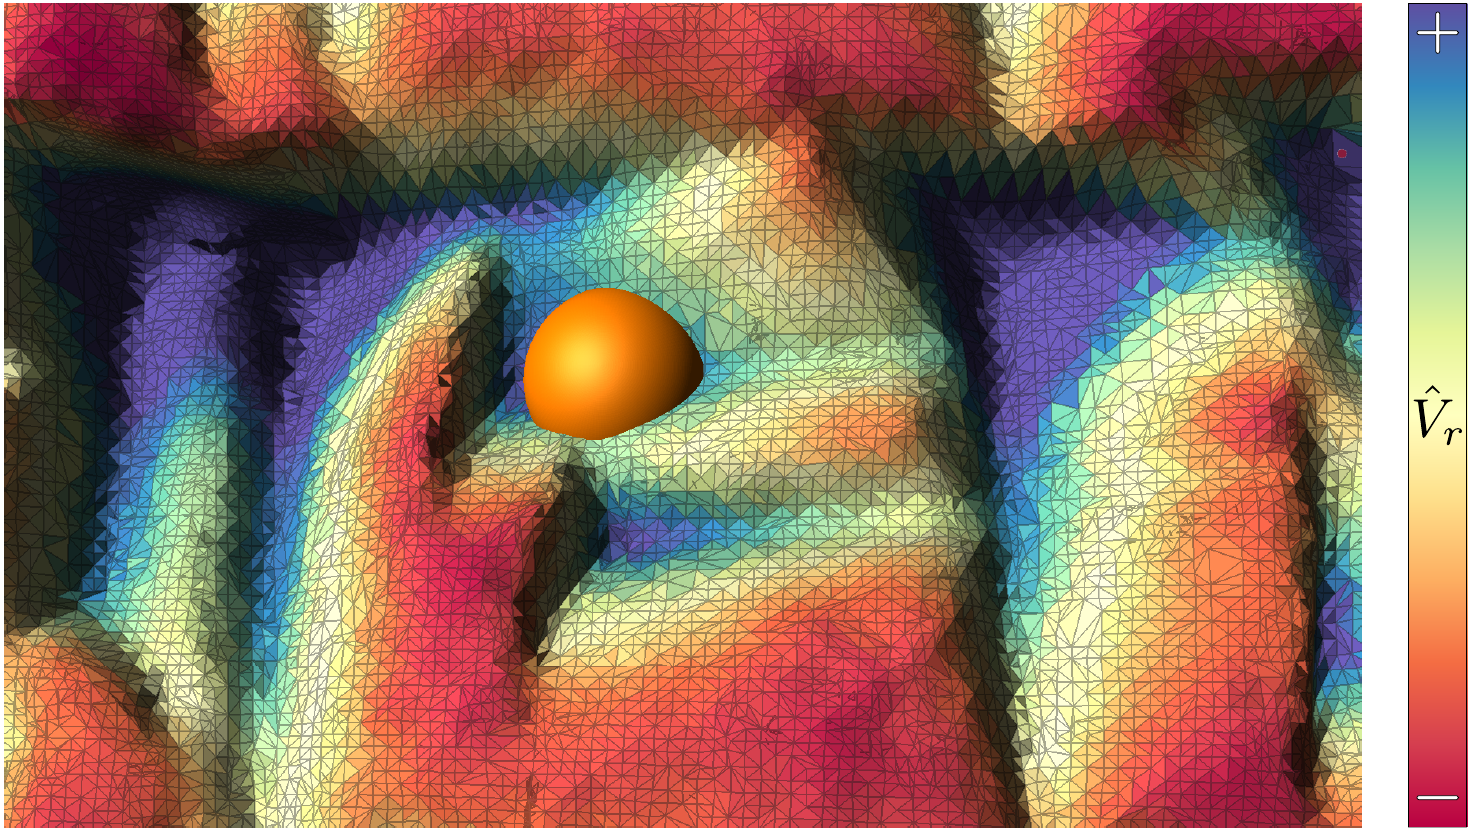
\includegraphics[width=1.0\linewidth]{figures/visualizeFunctionValues2.png}
			3D Surface Scan as a discrete 2D manifold \break colored by function value
		\end{column}
	\end{columns}
}

%------------------------------------------------
\frame{\frametitle{Raw \tdd{} is not suitable for analysis}
	\begin{columns}[T]
		\begin{column}{.45\textwidth}
			\begin{itemize}
				\item Non-manifold meshes, edges, and singular points
			\end{itemize}
			\begin{columns}[T]
				\begin{column}{.55\textwidth}
					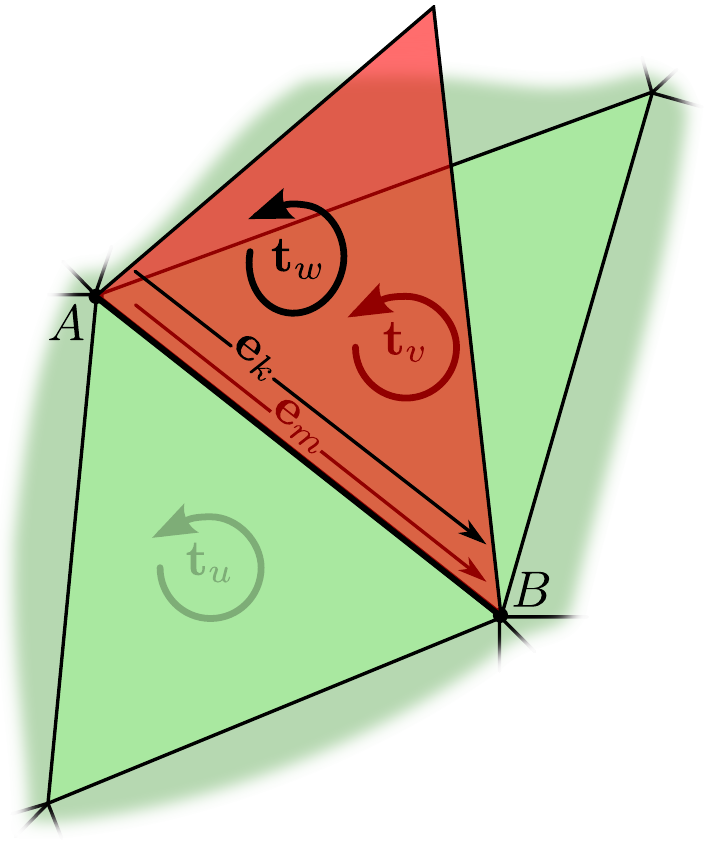
\includegraphics[width=\textwidth]{figures/badMesh3.png}
				\end{column}
				\begin{column}{.45\textwidth}
					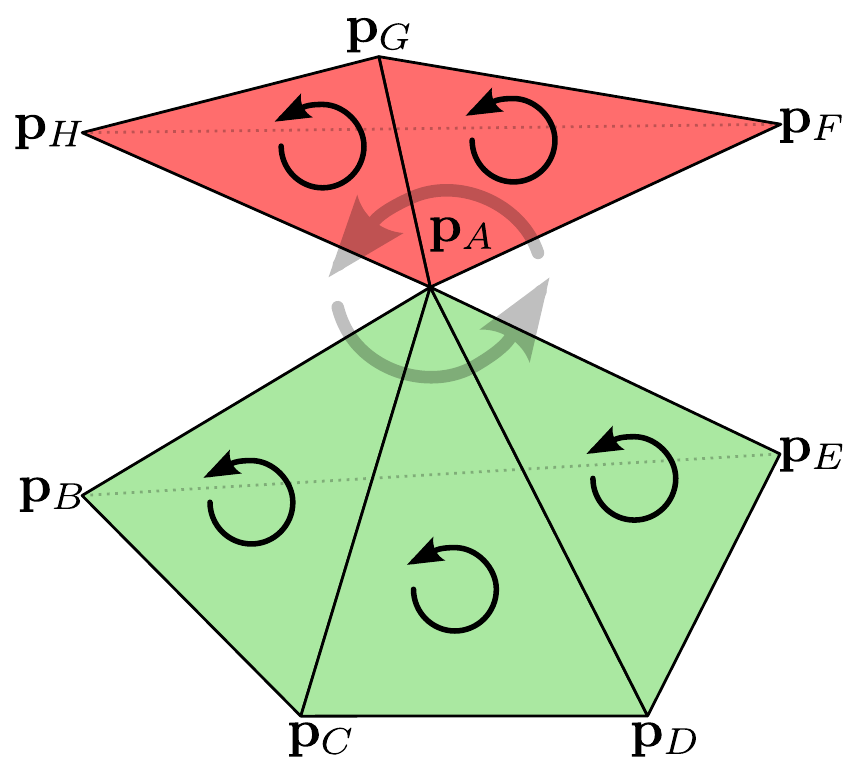
\includegraphics[width=\textwidth]{figures/badMesh1.png}
					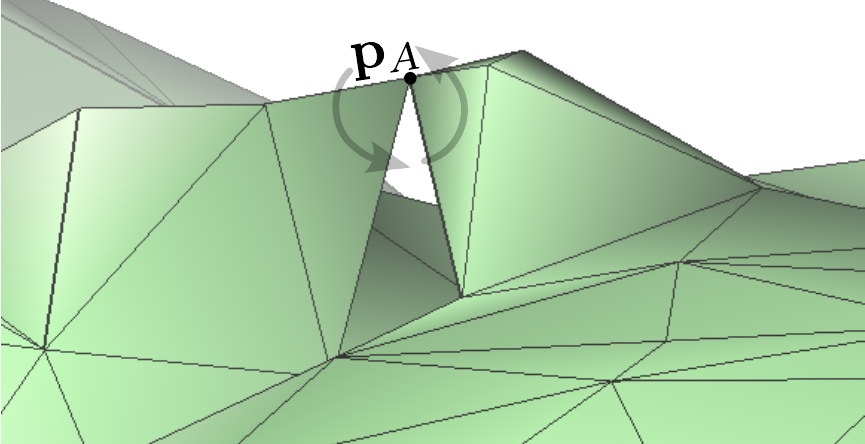
\includegraphics[width=\textwidth]{figures/badMesh2.png}
				\end{column}
			\end{columns}
		\end{column}
		\begin{column}{.475\textwidth}
			%\vspace*{4mm}
			\begin{itemize}
				\item Errors propagate in filter responses
				\item Jagged borders of segmented areas
			\end{itemize}
			\vspace*{4mm}
			\begin{columns}[T]
				\begin{column}{.1\textwidth}
				\end{column}
				\begin{column}{.45\textwidth}
					\centering
					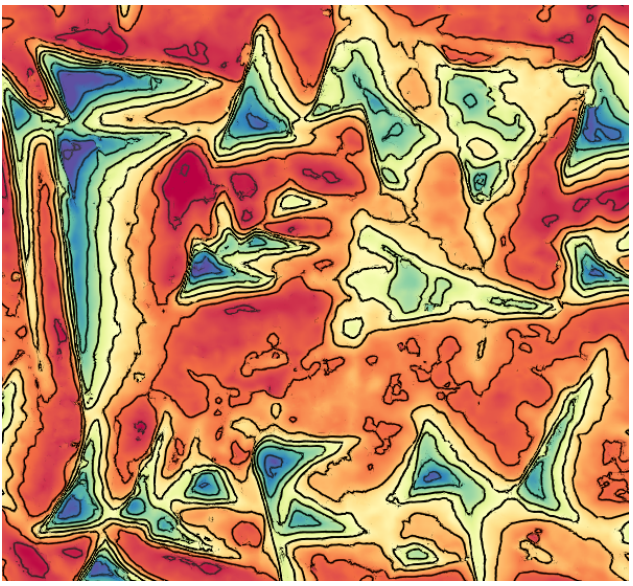
\includegraphics[width=\textwidth]{figures/beforeFilter.png}
					Before smoothing
				\end{column}
				\begin{column}{.45\textwidth}
					\centering
					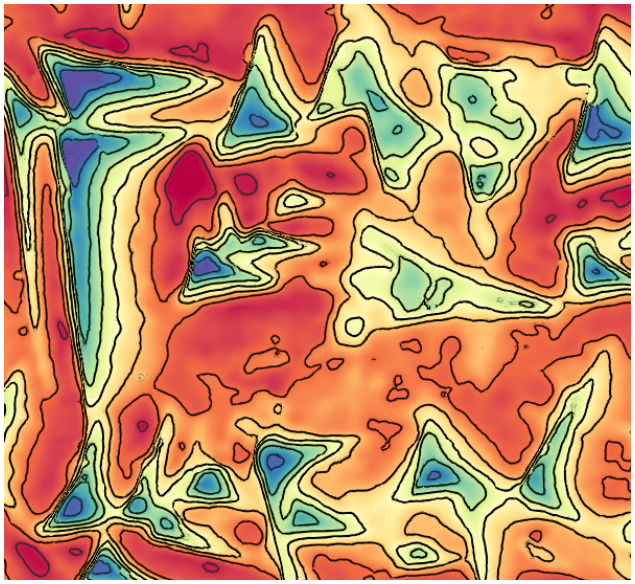
\includegraphics[width=\textwidth]{figures/afterFilter.png}
					After smoothing
				\end{column}
			\end{columns}
		\end{column}
	\end{columns}
}


%------------------------------------------------
\frame{\frametitle{Smoothing jagged borders of segmented areas}
	\vspace*{-4mm}
	\begin{columns}[T]
		\begin{column}{.5\textwidth}
			\centering
			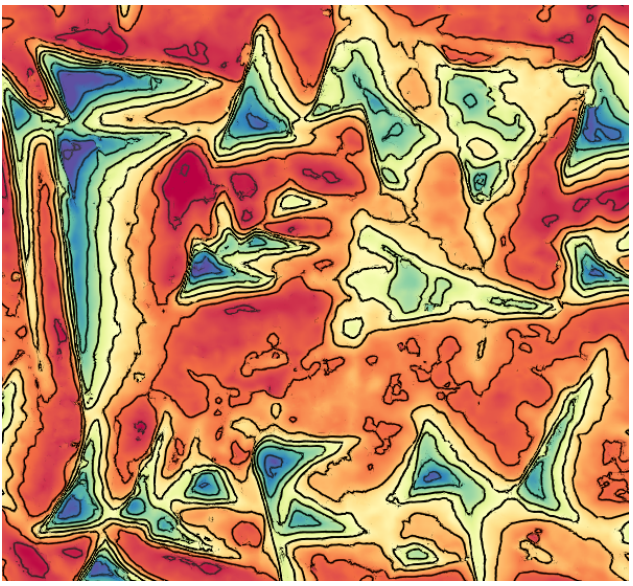
\includegraphics[width=.9\textwidth]{figures/beforeFilter.png}
			Before smoothing
		\end{column}
		\begin{column}{.5\textwidth}
			\centering
			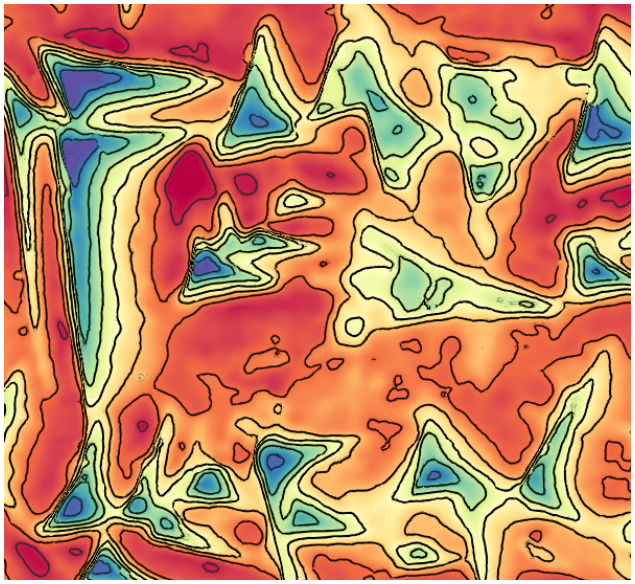
\includegraphics[width=.9\textwidth]{figures/afterFilter.png}
			After smoothing
		\end{column}
	\end{columns}
}

%------------------------------------------------
\frame{\frametitle{One-Ring Neighborhoods in Regular and Irregular Meshes}
	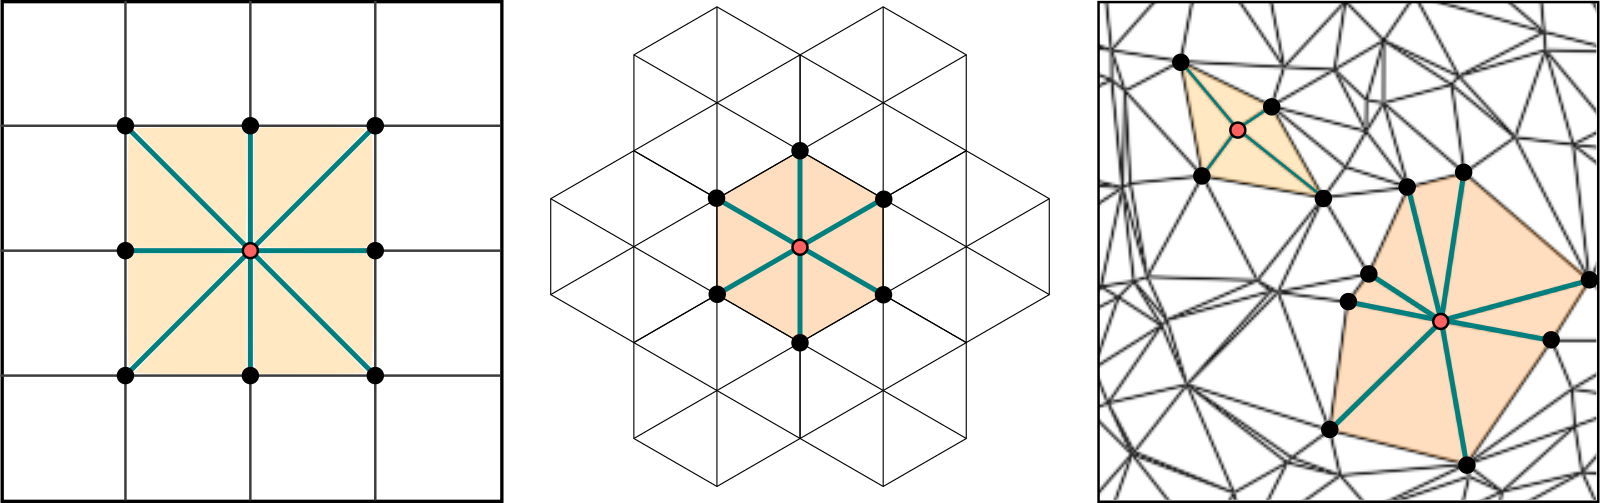
\includegraphics[width=1.0\linewidth]{figures/neighborhoods_presentation.png}

	\bigskip
	\begin{columns}[c]
		\begin{column}{.27\textwidth}
			a regular square mesh, as in pixels of a digital image
		\end{column}
		\begin{column}{.27\textwidth}
			a regular triangle mesh, as in a hexagonal tessellation
		\end{column}
		\begin{column}{.3\textwidth}
			an irregular triangle mesh, typical of acquired \tdd{}
		\end{column}
	\end{columns}
}
\fi
%------------------------------------------------
%TODO: format; add pictures?
\frame{\frametitle{Nomenclature}
	\begin{tabular}{ l l }
		$\bM$ & a mesh; a 2D discrete manifold in three dimensions \\
		$\bP$ & the set of points $\bp_v$ in $\bM$ \\
		$\bT$ & the set of faces $\bt_k$ in $\bM$ \\
		$\bF$ & the set of function values; the scalar field \\
		$\bN$ & the set of one-ring neighborhoods \\
		$\bN_v$ & a one-ring neighborhood of points \\
	\end{tabular}
}

\iffalse
%================================================
%================================================
\section{Fast One-Ring Smoothing}


%================================================
\subsection{Mathematical Foundation}

%------------------------------------------------
\frame{\frametitle{A One-Ring Neighborhood and its Geodesic Disc}
	\centering
	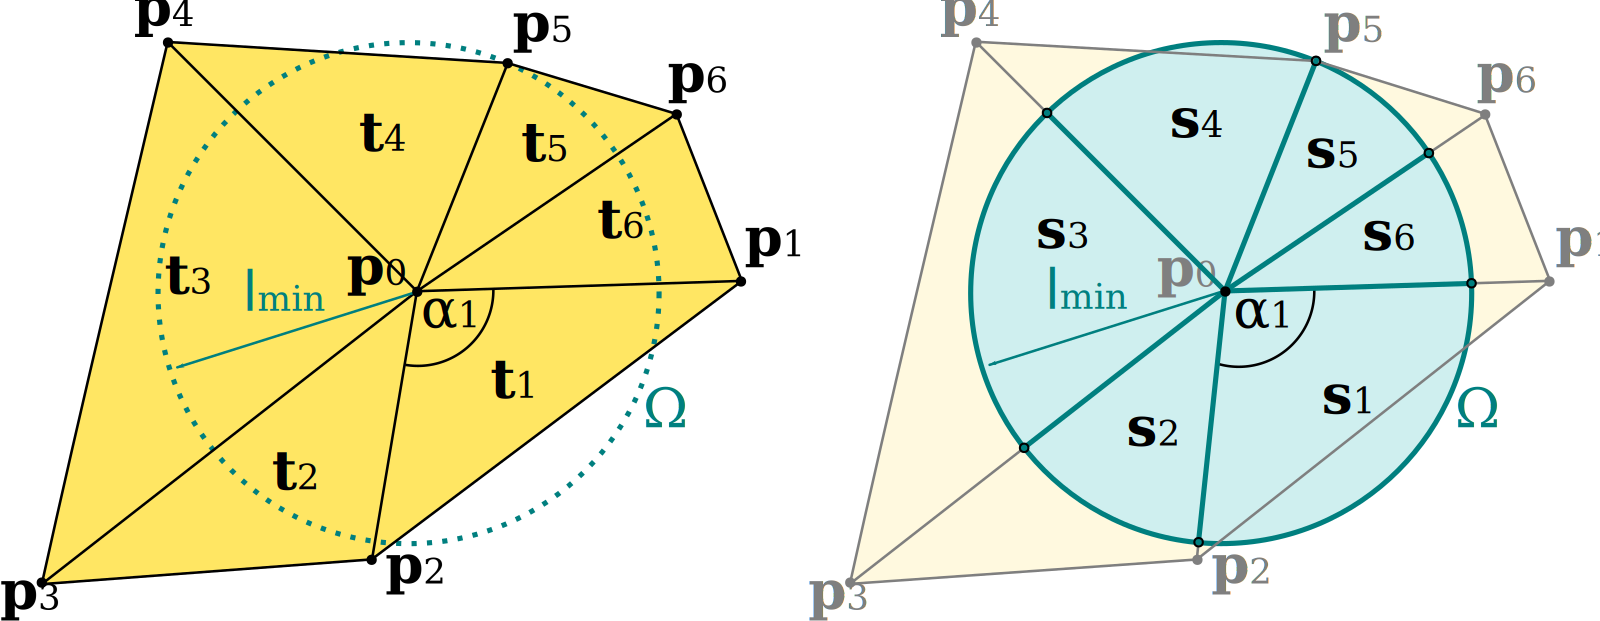
\includegraphics[width=0.8\linewidth]{figures/geodesicDisc_presentation.png}
	\begin{align*}
		\elm(\bp_0) &:= \min_{\forall \bp_i \in \bN_v}|\bp_i - \bp_0| \\
		\gelm &:= \min\left \{\elm(\bp_0) \;|\; \bp_0 \in \bM\,\right \}
	\end{align*}
}

%------------------------------------------------
%TODO:add math to Columns
\frame{\frametitle{An Enhanced View of a Circle Sector}
	\begin{columns}[T]
		\begin{column}{.5\textwidth}
			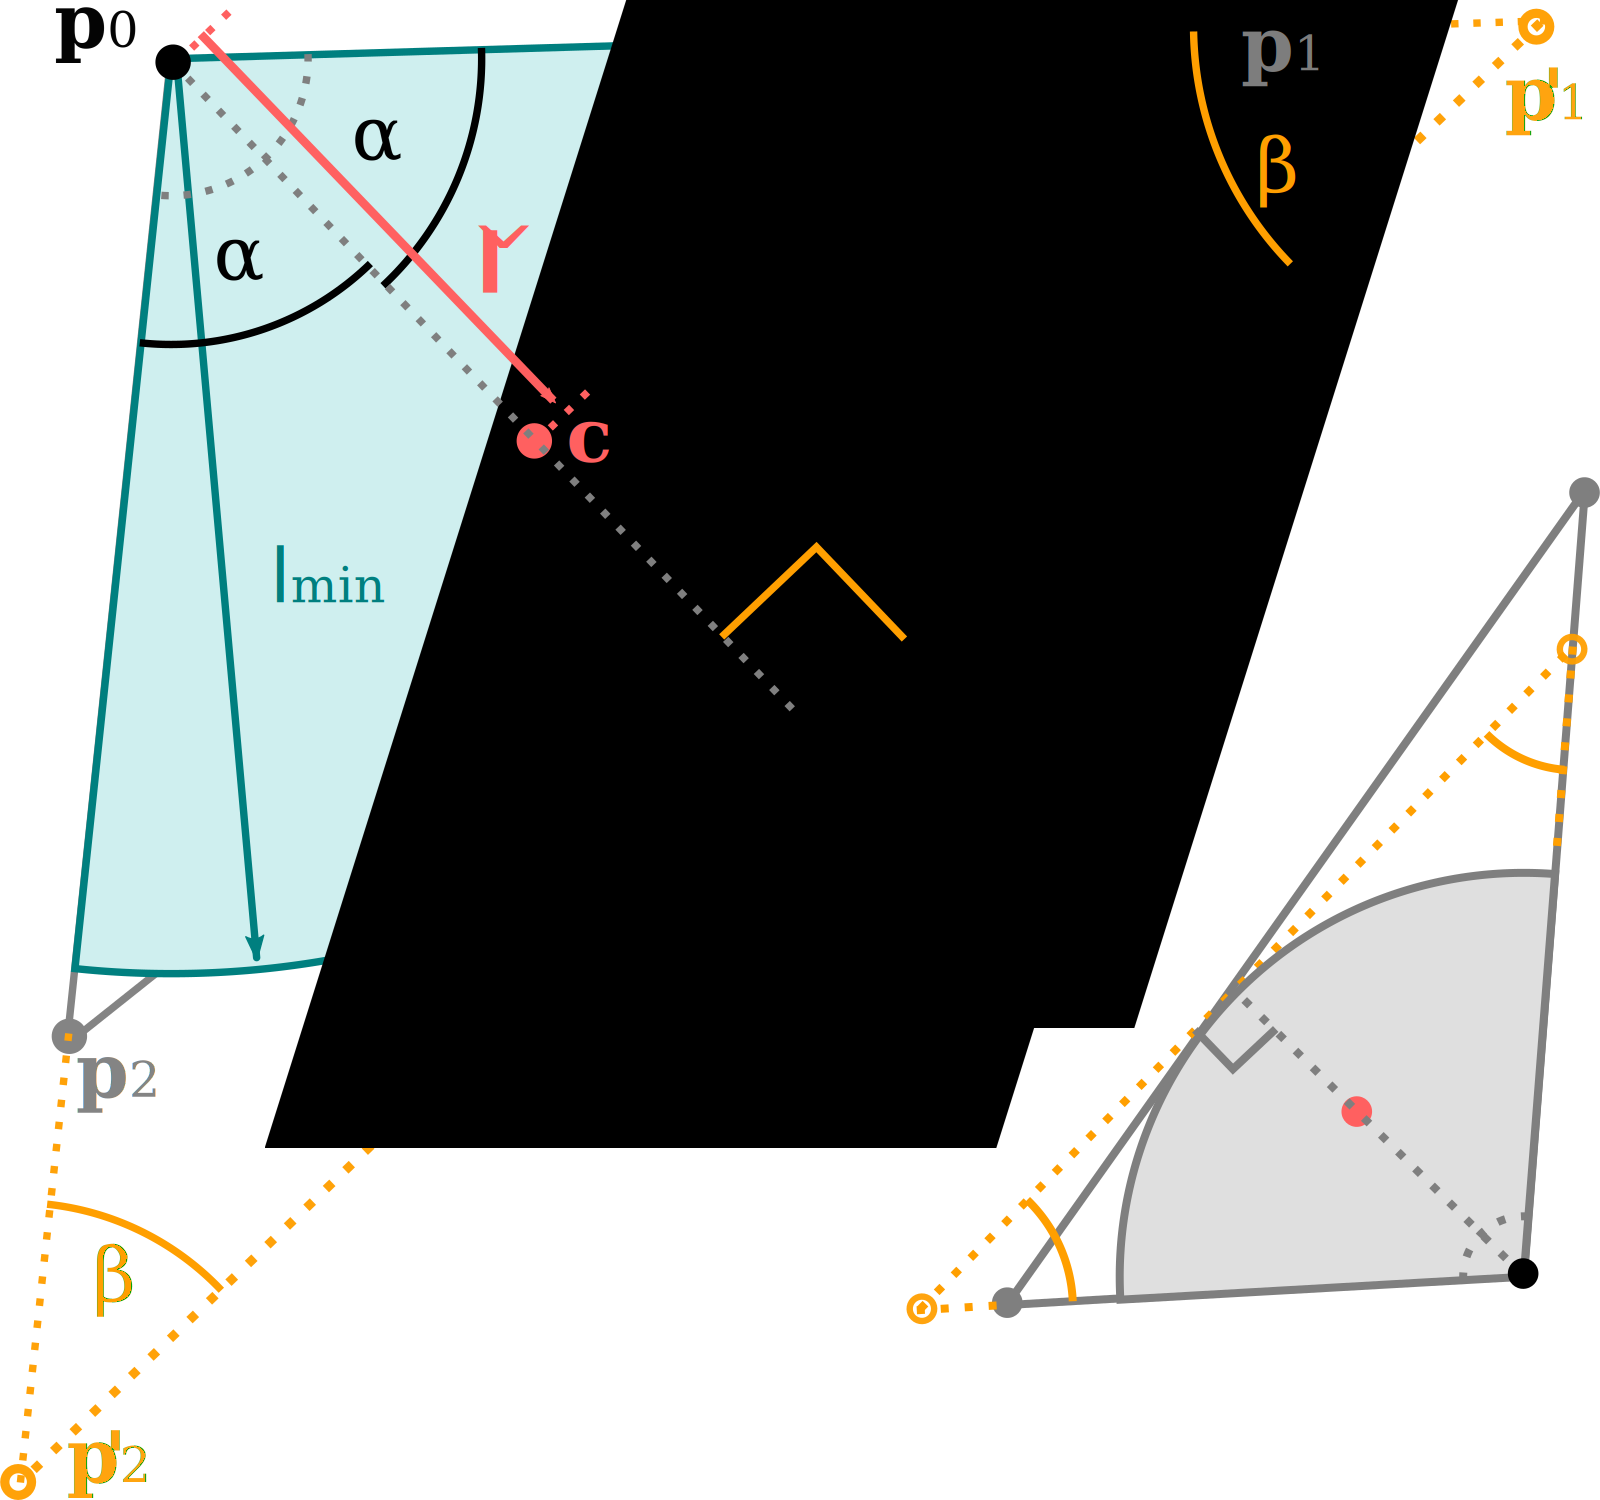
\includegraphics[width=\linewidth]{figures/anglesAndCenterOfGravity_presentation.png}
		\end{column}
		\begin{column}[t]{.5\textwidth}
			Math
			\begin{itemize}
				\item item 1
				\item item 1
				\item item 1
			\end{itemize}
		\end{column}
	\end{columns}
}

%------------------------------------------------
\frame{\frametitle{Interpolation of Function Values toward the Center of Gravity}
	\centering
	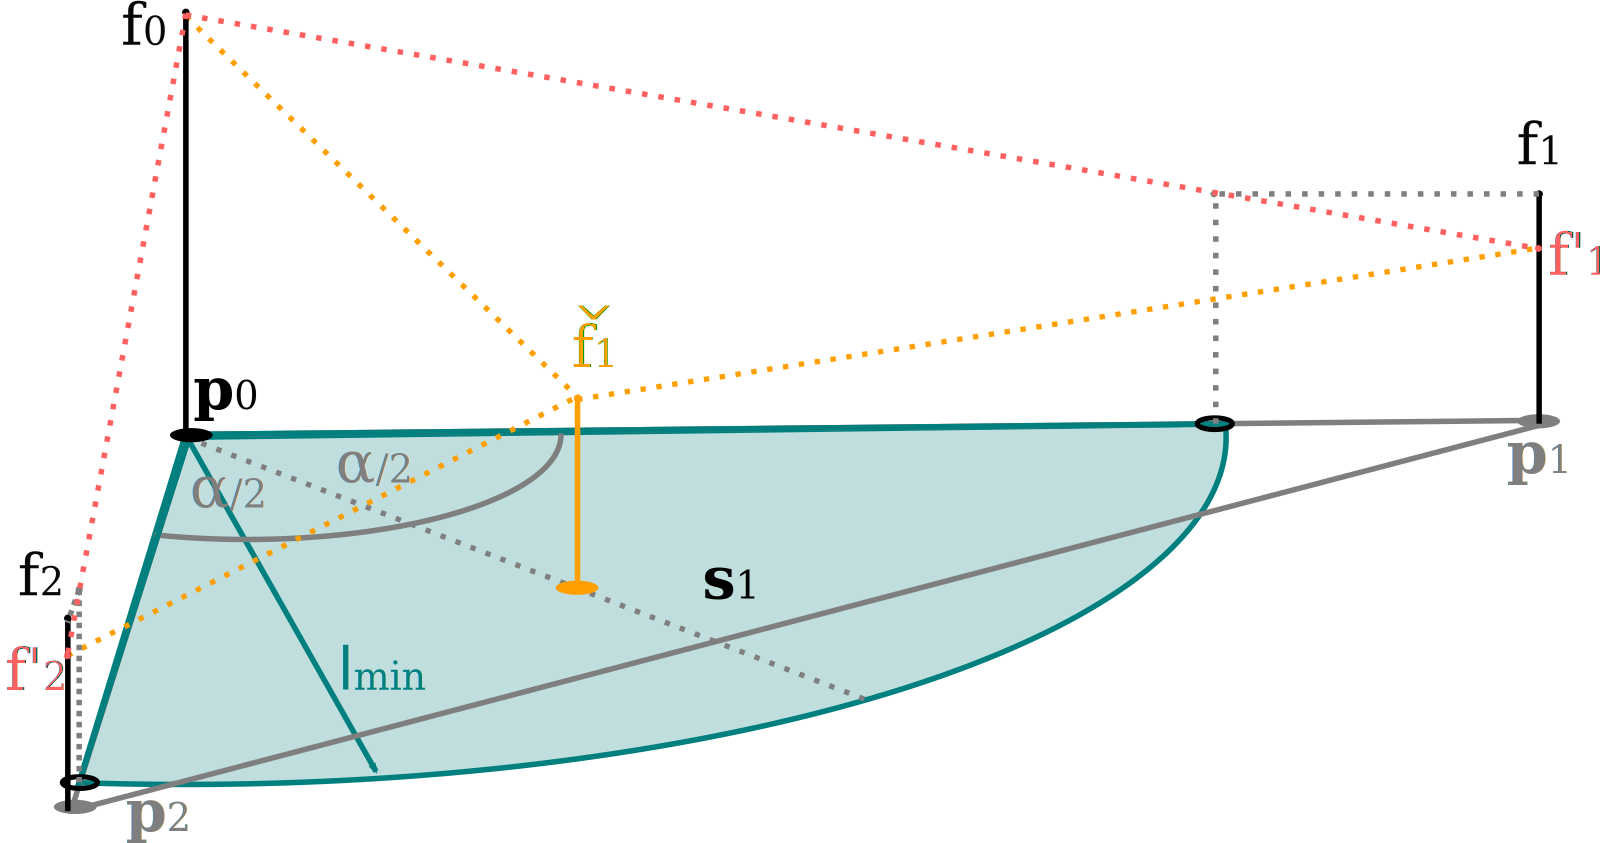
\includegraphics[width=0.95\linewidth]{figures/interpolatedFunctionValues.png}
}

%------------------------------------------------
\frame{\frametitle{Weighted Mean Function Value $f'_v$ at $\bp_v$}
	\vspace*{5mm}
	\centering
	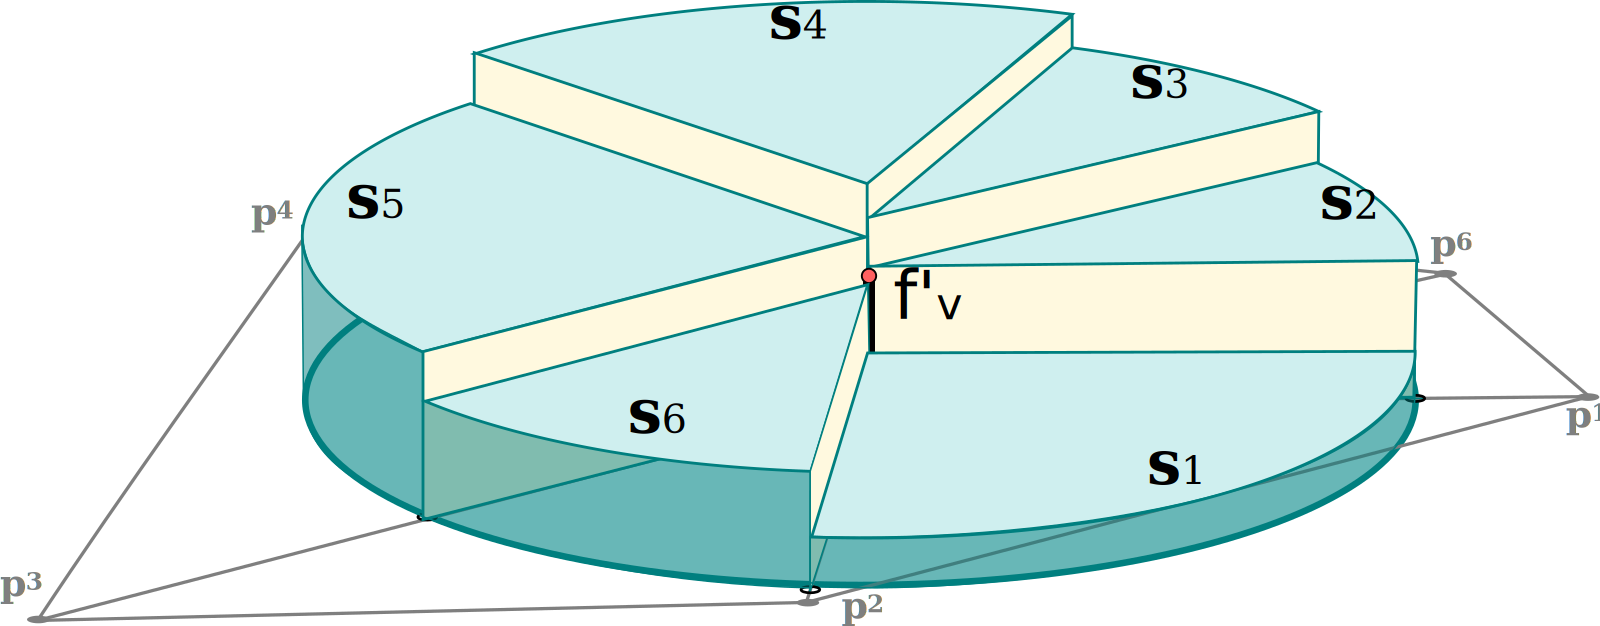
\includegraphics[width=1.0\linewidth]{figures/funcValVolumes_presentation.png}
}


%================================================
\subsection{Serial Algorithm}

%------------------------------------------------
\frame{\frametitle{Serial Algorithm for Building Neighborhoods}
	\begin{columns}[t]
		\begin{column}{.6\textwidth}
			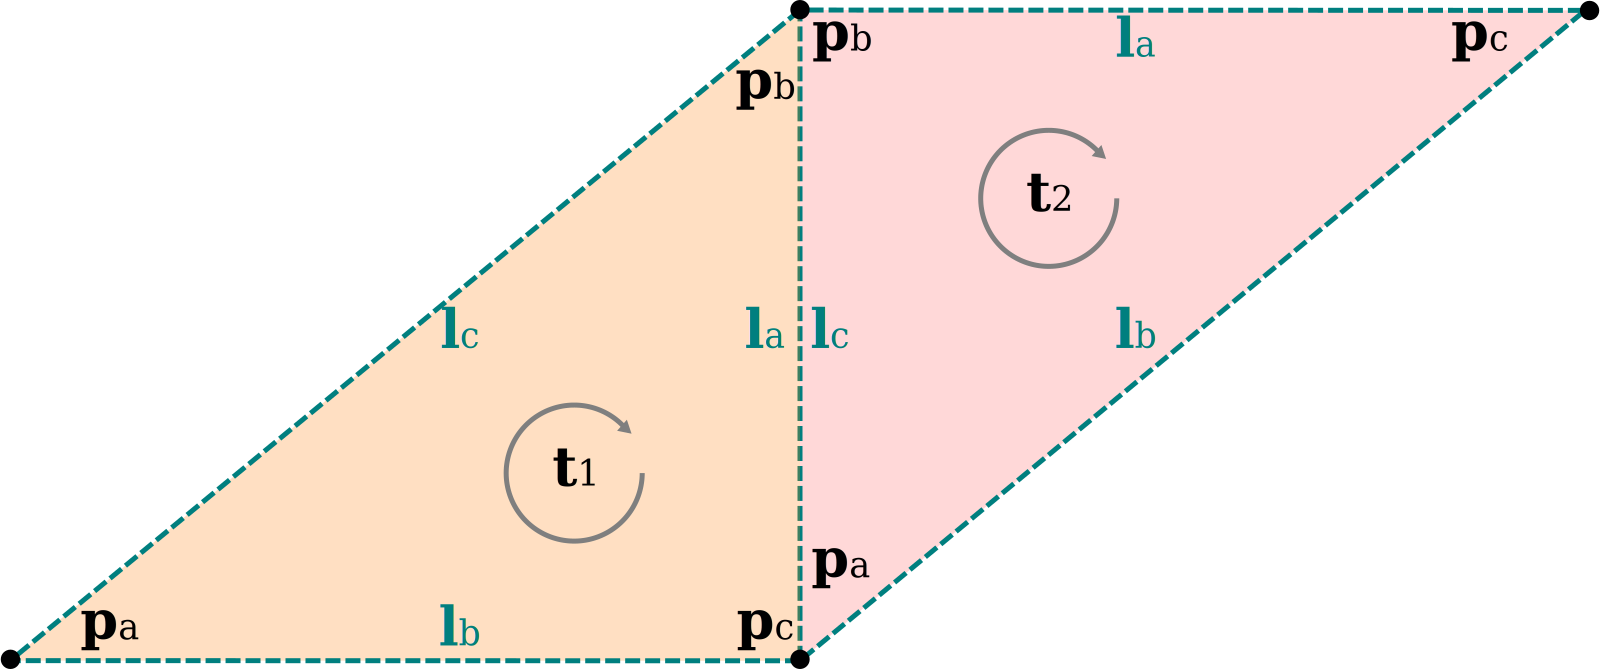
\includegraphics[width=1.0\linewidth]{figures/triangularFaces.png}
		\end{column}
		\hspace*{-1.5cm}
		\begin{column}{.6\textwidth}
			\includestandalone[width=1.0\linewidth]{figures/tikz/unionsOfSimpleBuildNeighborhoods}
		\end{column}
	\end{columns}

	\begin{columns}[t]
		\begin{column}{.5\textwidth}
			\begin{algorithm}[H]
				\DontPrintSemicolon
				\SetKwFor{For}{for}{:}{}
				\begin{block}{}
				\nl		\For{$\bt \in \bT$}{
				\nl			\ProgSty{union($\bN$, $\bp_a$, $\bp_b$, $\bp_c$)}\;
				\nl			\ProgSty{union($\bN$, $\bp_b$, $\bp_a$, $\bp_c$)}\;
				\nl			\ProgSty{union($\bN$, $\bp_c$, $\bp_a$, $\bp_b$)}\;
						}
				\end{block}
			\end{algorithm}
		\end{column}
		\begin{column}{.5\textwidth}
			\begin{algorithm}[H]
				\DontPrintSemicolon
				\SetKwFor{For}{for}{:}{}
				\SetKwProg{Func}{Function}{}{}
				\begin{block}{}
				\nl	\Func{union($\bN$, $a$, $b$, $c$)}{
				\nl		$\bN_a \leftarrow \bN_a \cup \{b,\,c\}$\;
					}
				\end{block}
			\end{algorithm}
		\end{column}
	\end{columns}
}

%------------------------------------------------
%TODO: Mention tau can be derived from feature size as in Mara17
\frame{\frametitle{Serial Algorithm for Calculating Edge Lengths}
\begin{algorithm}[H]
	\SetAlgoSkip{}
	\DontPrintSemicolon
	\SetCommentSty{small}
	\SetKwFor{For}{for}{:}{}
	\SetKwProg{Func}{Function}{}{}
	\SetKwInOut{Input}{Input}\SetKwInOut{Output}{Output}

	\only<1>{
	\begin{block}{}%Part (1 of 1)}
		\Input{the set of all points $\bP$, \\
			the set of discovered neighborhoods $\bN$}
		\Output{the set of pre-calculated edge lengths $\bE$, \\
			the minimum edge length of the mesh $\gelm$}

		\bigskip
	\nl	\Func{serialCalculateEdgeLengths($\bP$, $\bN$)}{
	\nl		\For{$\bp_v \in \bP$}{
	\nl			\For{$\bp_i \in \bN_v$}{
					\linespread{1.5}\selectfont
	\nl				$\bE_{\sv{i}} \leftarrow \lVert\bp_i - \bp_v\rVert_2$\tcc*[r]{\emph{Expensive!}}
	\nl				$\gelm \leftarrow \min\left \{\gelm,\,\bE_{\sv{i}}\right \}$\;
				}
			}
		}
	\end{block}
	}
\end{algorithm}
}

%------------------------------------------------
%TODO: be ready to translate symbols in part 3!
\frame{\frametitle{Serial Algorithm for Convolving the Filter}
	\vspace*{-8mm}
	\begin{columns}
		\begin{column}[t]{.35\textwidth}
			\begin{block}{}
				{\fontsize{4.2}{4.2}\selectfont
					\begin{algorithm}[H]
						\DontPrintSemicolon
						\SetCommentSty{small}
						\SetKwFor{For}{for}{:}{}
						\SetKwProg{Func}{Function}{}{}
						\SetKwProg{Cont}{}{}{}
						\SetKwInOut{Input}{Input}\SetKwInOut{Output}{Output}
						\Input{the set of all points $\bP$, \\
							the set of discovered neighborhoods $\bN$, \\
							the set of pre-calculated edge lengths $\bE$, \\
							the minimum edge length of the mesh $\gelm$, \\
							the set of function values $\bF$, \\
							the user-defined number of convolutions $\tau$}
						\Output{the set of one-ring \wmfv{s} $\bF'$}

						\medskip
						\linespread{1.2}\selectfont
					\nl	\Func{serialConvolveFilter($\bP$, $\bN$, $\bE$, $\gelm$, $\bF$, $\tau$)}{
					\nl		\For{$t\leftarrow 1\;\KwTo\;\tau$}{
					\nl			\For{$\bp_v \in \bP$}{
					\nl				\For{$\bp_i \in \bN_v$}{
										\linespread{1.5}\selectfont
					\nl					$\kern-0.5pt\alpha \leftarrow cos^{-1} \kern-6pt\left (\frac{\bE_c^2\,+\,\bE_b^2\,-\,\bE_a^2}{2\,\cdot\,\bE_c\,\cdot\,\bE_b}\right )$\;
										\linespread{1.2}\selectfont
					\nl					$\kern0.00pt\beta \leftarrow (\pi - \alpha)\mathbin{/}2$\;
					\nl					$\kern-1.5ptA \leftarrow \Big(\gelm\,\Big)^2\kern-4pt\cdot\alpha\mathbin{/}2$\;
					\nl					$\kern1.00pt\check{\ell} \leftarrow \big(4\cdot\gelm\cdot\sin(\alpha\mathbin{/}2)\big)\mathbin{/}3\,\alpha$\;
					\nl					$\kern1.00pt\zeta \leftarrow \gelm\mathbin{/}\sin(\beta)$\;
					\nl					\For{$j \in {1,2}$}{\label{algSCFjloop}
					\nl						$\tilde{\ell}_j \leftarrow \zeta\mathbin{/}\bE_j$\;
					\nl						$f'_j \leftarrow f_0\cdot(1 - \tilde{\ell}_j) + f_j\cdot\tilde{\ell}_j$\;
										}
					\nl					$\check{f} \leftarrow f_0\cdot(1 - \check{\ell}) + \big((f'_1 + f'_2)\cdot\check{\ell}\big)\mathbin{/}2$\;
					\nl					$\kern-2.0pt\tilde{f}_v \leftarrow \tilde{f}_v + A\cdot\check{f}$\;
					\nl					$\kern-4.0pt\tilde{A}_v \leftarrow \tilde{A}_v + A$\;
									}
					\nl				$f'_v \leftarrow \tilde{f}_v\mathbin{/}\tilde{A}_v$\;
								}
					\nl		$\bF' \leftarrow \left \{f'_1,\ldots,\,f'_{|\bP|}\right \}$\;
					\nl 	$\bF \leftarrow \bF'$\;
							}
						}
					\end{algorithm}
				}
			\end{block}
		\end{column}
		\begin{column}[t]{.65\textwidth}
			\only<1>{
				\begin{block}{Part (1 of 3)}
					\begin{algorithm}[H]
						\DontPrintSemicolon
						\SetCommentSty{small}
						\SetKwFor{For}{for}{:}{}
						\SetKwProg{Func}{Function}{}{}
						\SetKwProg{Cont}{}{}{}
						\SetKwInOut{Input}{Input}\SetKwInOut{Output}{Output}
						\Input{the set of all points $\bP$, \\
							the set of discovered neighborhoods $\bN$, \\
							the set of pre-calculated edge lengths $\bE$, \\
							the minimum edge length of the mesh $\gelm$, \\
							the set of function values $\bF$, \\
							the user-defined number of convolutions $\tau$}

						\bigskip
						\Output{the set of one-ring \wmfv{s} $\bF'$}
					\end{algorithm}
				\end{block}
			}\only<2>{
				\begin{block}{Part (2 of 3)}
					\begin{algorithm}[H]
						\SetAlgoLined
						\DontPrintSemicolon
						\SetCommentSty{small}
						\SetKwFor{For}{for}{:}{}
						\SetKwProg{Func}{Function}{}{}
						\SetKwProg{Cont}{}{}{}
						\setcounter{AlgoLine}{0}
					\nl	\Func{serialConvolveFilter($\bP$, $\bN$, $\bE$, $\gelm$, $\bF$, $\tau$)}{
					\nl		\For{$t\leftarrow 1\;\KwTo\;\tau$}{
					\nl			\For{$\bp_v \in \bP$}{
					\nl				\For{$\bp_i \in \bN_v$}{
										\vspace*{1.5\baselineskip}
										\ldots
										\vspace*{1.5\baselineskip}
									}
						\setcounter{AlgoLine}{15}
					\nl				$f'_v \leftarrow \tilde{f}_v\mathbin{/}\tilde{A}_v$\;
								}
					\nl		$\bF' \leftarrow \left \{f'_1,\ldots,\,f'_{|\bP|}\right \}$\;
					\nl 	$\bF \leftarrow \bF'$\;
							}
						}
					\end{algorithm}
				\end{block}
			}\only<3>{
				\begin{block}{Part (3 of 3)}
					{\fontsize{9}{9.5}\selectfont
					\begin{algorithm}[H]
						\SetAlgoLined
						\DontPrintSemicolon
						\SetCommentSty{small}
						\SetKwFor{For}{for}{:}{}
						\SetKwProg{Func}{Function}{}{}
						\SetKwProg{Cont}{}{}{}
						\setcounter{AlgoLine}{7}
						\vspace*{-1\baselineskip}
						\Cont{}{
							\vspace*{-1\baselineskip}
							\Cont{}{
								\vspace*{-1\baselineskip}
								\Cont{}{
									\vspace*{-1\baselineskip}
									\Cont{}{
										\linespread{1.5}\selectfont
					\nl					$\kern-0.5pt\alpha \leftarrow cos^{-1} \kern-6pt\left (\frac{\bE_c^2\,+\,\bE_b^2\,-\,\bE_a^2}{2\,\cdot\,\bE_c\,\cdot\,\bE_b}\right )$\;
										\linespread{1.2}\selectfont
					\nl					$\kern0.00pt\beta \leftarrow (\pi - \alpha)\mathbin{/}2$\;
					\nl					$\kern-1.5ptA \leftarrow \Big(\gelm\,\Big)^2\kern-4pt\cdot\alpha\mathbin{/}2$\;
					\nl					$\kern1.00pt\check{\ell} \leftarrow \big(4\cdot\gelm\cdot\sin(\alpha\mathbin{/}2)\big)\mathbin{/}3\,\alpha$\;
					\nl					$\kern1.00pt\zeta \leftarrow \gelm\mathbin{/}\sin(\beta)$\;
					\nl					\For{$j \in {1,2}$}{\label{algSCFjloop}
					\nl						$\tilde{\ell}_j \leftarrow \zeta\mathbin{/}\bE_j$\;
					\nl						$f'_j \leftarrow f_0\cdot(1 - \tilde{\ell}_j) + f_j\cdot\tilde{\ell}_j$\;
										}
					\nl					$\check{f} \leftarrow f_0\cdot(1 - \check{\ell}) + \big((f'_1 + f'_2)\cdot\check{\ell}\big)\mathbin{/}2$\;
					\nl					$\kern-2.0pt\tilde{f}_v \leftarrow \tilde{f}_v + A\cdot\check{f}$\;
					\nl					$\kern-4.0pt\tilde{A}_v \leftarrow \tilde{A}_v + A$\;
									}
								}
							}
						}
					\end{algorithm}
					}
				\end{block}
			}
		\end{column}
	\end{columns}
	\begin{tikzpicture}[overlay, remember picture]
		\draw<1>[unirot,ultra thick,rounded corners] (-8mm, 64mm) rectangle (46mm, 50mm);
		\draw<2>[unirot,ultra thick,rounded corners] (-8mm, 50mm) rectangle (46mm, 41mm);
		\draw<2>[unirot,ultra thick,rounded corners] (-8mm, 15mm) rectangle (46mm,  2mm);
		\draw<3>[unirot,ultra thick,rounded corners] (-8mm, 43mm) rectangle (46mm, 14mm);
	\end{tikzpicture}
}

%------------------------------------------------
\frame{\frametitle{SIMD Architecture}
	\includegraphics[width=1.0\linewidth]{figures/tikz/simdArchitecture.pdf}

	\bigskip
	\begin{flushright}
		i.e. GPUs, Supercomputers, Computer Pools %Name examples like the cray, and pool in this building
	\end{flushright}
}

%------------------------------------------------

\frame{\frametitle{CPU vs GPU Construction}
	\includegraphics[width=1.0\linewidth]{figures/cpuvgpu.png}
}


%================================================
\subsection{Data Dependencies}

%------------------------------------------------
\frame{\frametitle{Data Dependencies in Serial Algorithm Build Neighborhoods}
	\centering
	\includestandalone[width=0.725\textwidth]{figures/tikz/sabnDataDependencies}
}

%------------------------------------------------
\frame{\frametitle{Data Dependencies in Serial Algorithm Calculate Edge Lengths}
	\centering
	\includestandalone[width=0.875\textwidth]{figures/tikz/sacelDataDependencies}
}

%------------------------------------------------
%TODO: Overlapping memory nodes
\frame{\frametitle{Data Dependencies in Serial Algorithm Convolve Filter}
	\centering
	\includestandalone[width=0.4825\textwidth]{figures/tikz/sacfDataDependencies}
}


%================================================
\subsection{Parallel Algorithm}

%------------------------------------------------
\frame{\frametitle{Parallel Algorithm for Building Neighborhoods}
	\only<1>{
		\begin{block}{Part 1 of 3}
			\begin{algorithm}[H]
				\DontPrintSemicolon
				\SetKwFor{For}{for}{:}{}
				\SetKwProg{Func}{Function}{}{}
				\SetKwInOut{Input}{Input}\SetKwInOut{Output}{Output}

				\Input{the number of available processors $\rho$, \\
					the set of all triangular faces $\bT$, \\
					the cardinality of the set of points $|\bP|$}
				\Output{the set of discovered neighborhoods $\bN$}

				\bigskip
			\nl	\Func{parallelBuildNeighborhoods($\rho$, $\bT$, $|\bP|$)}{
			\nl		$\sigma \leftarrow |\bT|\mathbin{/}\rho$\;
			\nl		$\fM \leftarrow \{\mu_1,\,\ldots,\,\mu_{|\bP|}\}$\;
			\nl		\For{$\Pi \leftarrow 1$ \KwTo $\rho\mathbin{/}4$}{
			\nl			\ProgSty{$\sim$build($\Pi$, $\sigma$, $\fM$, $\bT$)}\;
					}
			\nl		\ProgSty{synchronizeThreads()}\;
				}
			\end{algorithm}
		\end{block}
	}
	\only<2>{
		\begin{columns}
			\begin{column}{.49\textwidth}
				\begin{block}{Part 2 of 3}
					\begin{algorithm}[H]
						\DontPrintSemicolon
						\SetCommentSty{small}
						\SetKwFor{For}{for}{:}{}
						\SetKwProg{Kernel}{Kernel}{}{}
						\setcounter{AlgoLine}{6}

					\nl	\Kernel{build($\Pi$, $\sigma$, $\fM$, $\bT$)}{
					\nl		$\check{\sigma} \leftarrow (\Pi-1)\,\sigma+1$\;
					\nl		$\hat{\sigma} \leftarrow \Pi\,\sigma$\;
					\nl		\For(\tcc*[f]{$\bt = \left \{\bp_a, \bp_b, \bp_c\right \}$}){$\bt \in \{\bt_{\check{\sigma}},\ldots,\,\bt_{\hat{\sigma}}\}$}{
					\nl			\ProgSty{$\sim$safeUnion($\fM$, $\bN$, $\bp_a$, $\bp_b$, $\bp_c$)}\;
					\nl			\ProgSty{$\sim$safeUnion($\fM$, $\bN$, $\bp_b$, $\bp_a$, $\bp_c$)}\;
					\nl			\ProgSty{$\sim$safeUnion($\fM$, $\bN$, $\bp_c$, $\bp_a$, $\bp_b$)}\;
							}
						}
					\end{algorithm}
				\end{block}
			\end{column}
			\begin{column}{.433\textwidth}
				\begin{block}{Part 3 of 3}
					\begin{algorithm}[H]
						\DontPrintSemicolon
						\SetCommentSty{small}
						\SetKwFor{For}{for}{:}{}
						\SetKwProg{Kernel}{Kernel}{}{}
						\setcounter{AlgoLine}{12}

					\nl	\Kernel{safeUnion($\fM$, $\bN$, $a$, $b$, $c$)}{
					\nl		$\ProcSty{lock}(\mu_a)$\;
					\nl		$\bN_a \leftarrow \bN_a \cup \{b,\,c\}$\;
					\nl		$\ProcSty{unlock}(\mu_a)$\;
						}
					\end{algorithm}
				\end{block}
			\end{column}
		\end{columns}
	}
}

%------------------------------------------------
%Totally remove
\iffalse
\frame{\frametitle{Parallel Recursive Census Neighborhoods (Prefix Sum)}
	\vspace*{-8mm}
	\begin{columns}
		\begin{column}{.49\textwidth}
			\begin{block}{}
				{\fontsize{5.8}{5.8}\selectfont
					\begin{algorithm}[H]
						\DontPrintSemicolon
						\SetCommentSty{small}
						\SetKwFor{For}{for}{:}{}
						\SetKwProg{Func}{Function}{}{}
						\SetKwProg{Kernel}{Kernel}{}{}
						\SetKwInOut{Input}{Input}\SetKwInOut{Output}{Output}

						\Input{the number of available processors $\rho$, \\
							the set of neighborhoods $\bN$}
						\Output{the count of all neighbors in all neighborhoods $\hat{n}$}

						\bigskip
					\nl	\Func{parallelRecursiveCensusNeighborhoods($\rho$, $\bN$)}{
					\nl		\eIf{$|\bN| \leq 2$}{
					\nl			$\hat{n} \leftarrow \sum_{i=1}^{|\bN|}\bN_i$\;
							}{%Else
					\nl			$\sigma \leftarrow |\bN|\mathbin{/}(2\,\rho)$\;
					\nl			\For{$\Pi \in \{1,\ldots,\rho\}$}{
					\nl				\ProgSty{$\sim$parallelSum($\Pi$, $\sigma$, $\bN$)}\;
								}
					\nl			\ProgSty{synchronizeThreads()}\;
					\nl			\ProgSty{parallelRecursiveCensusNeighborhoods($\rho$, $\widetilde{\bN}$)}\;
							}
						}

						\bigskip
					\nl	\Kernel{parallelSum($\Pi$, $\sigma$, $\bN$)}{
					\nl		$\check{\sigma} \leftarrow (\Pi-1)\,\sigma+1$\;
					\nl		$\hat{\sigma} \leftarrow 2\,\Pi\,\sigma$\;
					\nl		\For{$v \in \{\check{\sigma},\,\check{\sigma}\sps{}2,\,\check{\sigma}\sps{}4,\ldots,\,\hat{\sigma}\}$}{
					\nl			\eIf{$\bN$ is a family of sets}{
					\nl				$\widetilde{\bN_v} \leftarrow |\bN_v| + |\bN_{\sxpx{v}{1}}|$\;
								}{%else
					\nl				$\widetilde{\bN_v} \leftarrow \bN_v + \bN_{\sxpx{v}{1}}$\;
								}
							}
						}
					\end{algorithm}
				}
			\end{block}
		\end{column}
	\end{columns}
}
\fi
%------------------------------------------------
\frame{\frametitle{Parallel Algorithm for Calculating Edge Lengths}
	\vspace*{-8mm}
	\begin{columns}
		\begin{column}[t]{.35\textwidth}
			\begin{block}{}
				{\fontsize{4.2}{4.2}\selectfont
					\begin{algorithm}[H]
						\DontPrintSemicolon
						\SetCommentSty{small}
						\SetKwFor{For}{for}{:}{}
						\SetKwProg{Func}{Function}{}{}
						\SetKwProg{Kernel}{Kernel}{}{}
						\SetKwInOut{Input}{Input}\SetKwInOut{Output}{Output}

						\Input{the number of available processors $\rho$, \\
							the set of all points $\bP$, \\
							the set of neighborhoods $\bN$, \\
							the count of all neighbors in all neighborhoods $\hat{n}$}
						\Output{the set of pre-calculated edge lengths $\bE$, \\
							the global minimum edge length $\gelm$}

						\medskip
					\nl	\Func{parallelCalculateEdgeLengths($\rho$, $\bP$,\,$\bN$,\,$\hat{n}$)}{
					\nl		$\sigma \leftarrow \hat{n}\mathbin{/}\rho$\;
					\nl		$\bar{n} \leftarrow \hat{n}\mathbin{/}|\bP|$\;
					\nl		\For{$\Pi \in \{1,\,\ldots,\,\left \lceil\rho/\bar{n}\right\rceil\}$}{
					\nl			\ProgSty{$\sim$calculateLengths($\Pi$, $\sigma$, $\mu$, $\bP$,\,$\bN$)}\;
							}
					\nl		\ProgSty{synchronizeThreads()}\;
						}

						\medskip
					\nl	\Kernel{calculateLengths($\Pi$, $\sigma$, $\bP$,\,$\bN$)}{
					\nl		$\check{\sigma} \leftarrow (\Pi-1)\,\sigma+1$\;
					\nl		$\hat{\sigma} \leftarrow \Pi\,\sigma$\;
					\nl		$\ProcSty{create}(\mu)$\;
					\nl		\For{$\bp_v \in \{\bp_{\check{\sigma}},\ldots,\,\bp_{\hat{\sigma}}\}$}{
					\nl			\For{$\bp_i \in \bN_v$}{
					\nl				\ProgSty{$\sim$safeEdgeLengthCalc($\mu$, $\bE$, $\gelm$, $\bp_v$, $\bp_i$)}\;
								}
							}
						}

						\medskip
					\nl	\Kernel{safeEdgeLengthCalc($\mu$, $\bE$, $\gelm$, $\bp_v$, $\bp_i$)}{
					\nl		$\bE_{\sv{i}} \leftarrow |\bp_i - \bp_v|$\;
					\nl		\If{$\bE_{\sv{i}} < \gelm$}{\label{algPCELhcs}
					\nl			$\ProcSty{lock}(\mu)$\;
					\nl			$\gelm \leftarrow \min\left \{\gelm,\,\bE_{\sv{i}}\right \}$\label{algPCELgelm}\;
					\nl			$\ProcSty{unlock}(\mu)$\;
							}
						}
					\end{algorithm}
				}
			\end{block}
		\end{column}
		\begin{column}[t]{.65\textwidth}
			\only<1>{
				\begin{block}{Part (1 of 4)}
					\begin{algorithm}[H]
						\DontPrintSemicolon
						\SetKwInOut{Input}{Input}\SetKwInOut{Output}{Output}
						\Input{the number of available processors $\rho$, \\
							the set of all points $\bP$, \\
							the set of neighborhoods $\bN$, \\
							{\fontsize{9.5}{9.5}\selectfont the count of all neighbors in all neighborhoods $\hat{n}$}}

						\bigskip
						\Output{the set of pre-calculated edge lengths $\bE$, \\
							the global minimum edge length $\gelm$}
					\end{algorithm}
				\end{block}
			}\only<2>{
				\begin{block}{Part (2 of 4)}
					\begin{algorithm}[H]
						\DontPrintSemicolon
						\SetKwFor{For}{for}{:}{}
						\SetKwProg{Func}{Function}{}{}
						\setcounter{AlgoLine}{0}
					\nl	\Func{parallelCalculateEdgeLengths($\rho$, $\bP$,\,$\bN$,\,$\hat{n}$)}{
					\nl		$\sigma \leftarrow \hat{n}\mathbin{/}\rho$\;
					\nl		$\bar{n} \leftarrow \hat{n}\mathbin{/}|\bP|$\;
					\nl		\For{$\Pi \in \{1,\,\ldots,\,\left \lceil\rho/\bar{n}\right\rceil\}$}{
					\nl			\ProgSty{$\sim$calculateLengths($\Pi$, $\sigma$, $\mu$, $\bP$,\,$\bN$)}\;
							}
					\nl		\ProgSty{synchronizeThreads()}\;
						}
					\end{algorithm}
				\end{block}
			}\only<3>{
				\begin{block}{Part (3 of 4)}
					\begin{algorithm}[H]
						\DontPrintSemicolon
						\SetCommentSty{small}
						\SetKwFor{For}{for}{:}{}
						\SetKwProg{Kernel}{Kernel}{}{}
						\setcounter{AlgoLine}{6}
					\nl	\Kernel{calculateLengths($\Pi$, $\sigma$, $\bP$,\,$\bN$)}{
					\nl		$\check{\sigma} \leftarrow (\Pi-1)\,\sigma+1$\;
					\nl		$\hat{\sigma} \leftarrow \Pi\,\sigma$\;
					\nl		$\ProcSty{create}(\mu)$\;
					\nl		\For{$\bp_v \in \{\bp_{\check{\sigma}},\ldots,\,\bp_{\hat{\sigma}}\}$}{
					\nl			\For{$\bp_i \in \bN_v$}{
					\nl				\ProgSty{$\sim$safeEdgeLengthCalc($\mu$, $\bE$, $\gelm$, $\bp_v$, $\bp_i$)}\;
								}
							}
						}
					\end{algorithm}
				\end{block}
			}\only<4>{
				\begin{block}{Part (4 of 4)}
					\begin{algorithm}[H]
						\DontPrintSemicolon
						\SetCommentSty{small}
						\SetKwFor{For}{for}{:}{}
						\SetKwProg{Kernel}{Kernel}{}{}
						\setcounter{AlgoLine}{12}
					\nl	\Kernel{safeEdgeLengthCalc($\mu$, $\bE$, $\gelm$, $\bp_v$, $\bp_i$)}{
					\nl		$\bE_{\sv{i}} \leftarrow |\bp_i - \bp_v|$\;
					\nl		\If{$\bE_{\sv{i}} < \gelm$}{\label{algPCELhcs}
					\nl			$\ProcSty{lock}(\mu)$\;
					\nl			$\gelm \leftarrow \min\left \{\gelm,\,\bE_{\sv{i}}\right \}$\label{algPCELgelm}\;
					\nl			$\ProcSty{unlock}(\mu)$\;
							}
						}
					\end{algorithm}
				\end{block}
			}
		\end{column}
	\end{columns}
	\begin{tikzpicture}[overlay, remember picture]
		\draw<1>[unirot,ultra thick,rounded corners] (-8mm, 64mm) rectangle (46mm, 52mm);
		\draw<2>[unirot,ultra thick,rounded corners] (-8mm, 52.5mm) rectangle (46mm, 38.5mm);
		\draw<3>[unirot,ultra thick,rounded corners] (-8mm, 38mm) rectangle (46mm, 20mm);
		\draw<4>[unirot,ultra thick,rounded corners] (-8mm, 20mm) rectangle (46mm, 02mm);
	\end{tikzpicture}
}

%------------------------------------------------
%TODO: format
\frame{\frametitle{Parallel Algorithm for Convolving the Filter}
	\vspace*{-8mm}
	\begin{columns}
		\begin{column}[t]{.35\textwidth}
			\begin{block}{}
				{\scalebox{.66}{\fontsize{4.0}{4.0}\selectfont
					\begin{algorithm}[H]
						\DontPrintSemicolon
						\SetCommentSty{small}
						\SetKwFor{For}{for}{:}{}
						\SetKwProg{Func}{Function}{}{}
						\SetKwProg{Kernel}{Kernel}{}{}
						\SetKwInOut{Input}{Input}\SetKwInOut{Output}{Output}

						\Input{the number of available processors $\rho$, \\
							the set of all points $\bP$, \\
							the set of neighborhoods $\bN$, \\
							the count of all neighbors in all neighborhoods $\hat{n}$, \\
							the set of pre-calculated edge lengths $\bE$, \\
							the global minimum edge length $\gelm$, \\
							the set of function values $\bF$, \\
							the user-defined number of convolutions $\tau$}
						\Output{the set of one-ring \wmfv{s} $\bF'$}

						\smallskip
						\linespread{1}\selectfont
					\nl	\Func{parallelConvolveFilter($\rho$, $\bP$, $\bN$, $\hat{n}$, $\bE$, $\gelm$, $\bF$, $\tau$)}{
					\nl		\For{$t\leftarrow 1\;\KwTo\;\tau$}{
					\nl			$\sigma \leftarrow (|\bP|+\hat{n})\mathbin{/}\rho$\;
					\nl			$\bar{n} \leftarrow \tilde{n}\mathbin{/}|\bP|$\;
					\nl			\For{$\Pi \in \{1,\ldots,\left \lceil\rho/\bar{n}\right\rceil\}$}{
					\nl				\ProgSty{$\sim$safeAccumulateGeoDiscMean($\Pi$, $\sigma$, $\bP$, $\bN$, $\bE$, $\gelm$, $\bF$, $\bF'$)}\;
								}
					\nl			\ProgSty{synchronizeThreads()}\;
					\nl 		\If{$t < \tau$}{$\bF \leftarrow \bF'$}
							}
					\nl 	\KwRet $\bF'$\;
						}

						\smallskip
					\nl	\Kernel{safeAccumulateGeoDiscMean($\Pi$, $\sigma$, $\bP$, $\bN$, $\bE$, $\gelm$, $\bF$, $\bF'$)}{
					\nl		$\check{\sigma} \leftarrow (\Pi-1)\,\sigma+1$\;
					\nl		$\hat{\sigma} \leftarrow \Pi\,\sigma$\;
					\nl		\For{$\bp_v \in \{\bp_{\check{\sigma}},\ldots,\,\bp_{\hat{\sigma}}\}$}{
					\nl			$\fM \leftarrow \left \{\mu_1,\dots,\mu_{|\bN_v|}\right \}$\;
					\nl			\For{$\bp_i \in \bN_v$}{
									\smallskip
					\nl				\ProgSty{$\sim$safeAccumulateSectorMean($\fM$, $\bE$, $\gelm$, $\bp_v$, $\bp_i$, $\bF$, $\tilde{f}_v$, $\tilde{A}_v$)}\;
								}
					\nl			\ProgSty{synchronizeThreads(\{$\check{\sigma}$, \ldots, $\hat{\sigma}$\})}\;
					\nl			$\bF'_v \leftarrow \tilde{f}_v\mathbin{/}\tilde{A}_v$\;
							}
						}

						\smallskip
					\nl	\Kernel{safeAccumulateSectorMean($\fM$, $\bE$, $\gelm$, $\bp_v$, $\bp_i$, $\bF$, $\tilde{f}_v$, $\tilde{A}_v$)}{
					\nl		$\kern-0.5pt\alpha \leftarrow cos^{-1}\kern-6pt\left (\frac{\bE_c^2\,+\,\bE_b^2\,-\,\bE_a^2}{2\,\cdot\,\bE_c\,\cdot\,\bE_b}\right )$\;
					\nl		$\kern0.00pt\beta \leftarrow (\pi - \alpha)\mathbin{/}2$\;
					\nl		$\kern-1.5ptA \leftarrow \Big(\gelm\,\Big)^2\kern-4pt\cdot\alpha\mathbin{/}2$\;
					\nl		$\kern1.00pt\check{\ell} \leftarrow \big(4\cdot\gelm\cdot\sin(\alpha\mathbin{/}2)\big)\mathbin{/}3\,\alpha$\;
					\nl		$\kern1.00pt\zeta \leftarrow \gelm\mathbin{/}\sin(\beta)$\;
					\nl		\For{$j \in {1,2}$}{
					\nl			$\tilde{\ell}_j \leftarrow \zeta\mathbin{/}\bE_j$\;
					\nl			$f'_j \leftarrow f_0\cdot(1 - \tilde{\ell}_j) + f_j\cdot\tilde{\ell}_j$\;
							}
					\nl		$\check{f} \leftarrow f_0\cdot(1 - \check{\ell}) + \big((f'_1 + f'_2)\cdot\check{\ell}\big)\mathbin{/}2$\;
							\linespread{1.0}\selectfont
					\nl		$\ProcSty{lock}(\mu)$\;
					\nl		$\kern2.0pt\tilde{f}_v \leftarrow \tilde{f}_v + A\cdot\check{f}$\;
					\nl		$\kern0.0pt\tilde{A}_v \leftarrow \tilde{A}_v + A$\;
					\nl		$\ProcSty{lock}(\mu)$\;
						}
					\end{algorithm}
				}}
			\end{block}
		\end{column}
		\begin{column}[t]{.65\textwidth}
			\only<1>{
				\begin{block}{Part (1 of 4)}
					\begin{algorithm}[H]
						\DontPrintSemicolon
						\SetKwInOut{Input}{Input}\SetKwInOut{Output}{Output}
						\Input{the number of available processors $\rho$, \\
							the set of all points $\bP$, \\
							the set of neighborhoods $\bN$, \\
							{\fontsize{9.5}{9.5}\selectfont the count of all neighbors in all neighborhoods $\hat{n}$}, \\
							the set of pre-calculated edge lengths $\bE$, \\
							the global minimum edge length $\gelm$, \\
							the set of function values $\bF$, \\
							the user-defined number of convolutions $\tau$}

						\bigskip
						\Output{the set of one-ring \wmfv{s} $\bF'$}
					\end{algorithm}
				\end{block}
			}
			\only<2>{
				\begin{block}{Part (2 of 4)}
					{\fontsize{10}{12}\selectfont
					\begin{algorithm}[H]
						\DontPrintSemicolon
						\SetKwFor{For}{for}{:}{}
						\SetKwProg{Func}{Function}{}{}
						\setcounter{AlgoLine}{0}

					\nl	\Func{parallelConvolveFilter($\rho$, $\bP$, $\bN$, $\hat{n}$, $\bE$, $\gelm$, $\bF$, $\tau$)}{
					\nl		\For{$t\leftarrow 1\;\KwTo\;\tau$}{
					\nl			$\sigma \leftarrow (|\bP|+\hat{n})\mathbin{/}\rho$\;
					\nl			$\bar{n} \leftarrow \tilde{n}\mathbin{/}|\bP|$\;
					\nl			\For{$\Pi \in \{1,\ldots,\left \lceil\rho/\bar{n}\right\rceil\}$}{
					\nl				\ProgSty{$\sim$safeAccumulateGeoDiscMean($\Pi$, $\sigma$, $\bP$, $\bN$, $\bE$, $\gelm$, $\bF$, $\bF'$)}\;
								}
					\nl			\ProgSty{synchronizeThreads()}\;
					\nl 		\If{$t < \tau$}{$\bF \leftarrow \bF'$}
							}
					\nl 	\KwRet $\bF'$\;
						}
					\end{algorithm}
					}
				\end{block}
			}\only<3>{
				\begin{block}{Part (3 of 4)}
					{\fontsize{10}{12}\selectfont
					\begin{algorithm}[H]
						\DontPrintSemicolon
						\SetKwFor{For}{for}{:}{}
						\SetKwProg{Kernel}{Kernel}{}{}
						\setcounter{AlgoLine}{9}

					\nl	\Kernel{safeAccumulateGeoDiscMean($\Pi$, $\sigma$, $\bP$, $\bN$, $\bE$, $\gelm$, $\bF$, $\bF'$)}{
					\nl		$\check{\sigma} \leftarrow (\Pi-1)\,\sigma+1$\;
					\nl		$\hat{\sigma} \leftarrow \Pi\,\sigma$\;
					\nl		\For{$\bp_v \in \{\bp_{\check{\sigma}},\ldots,\,\bp_{\hat{\sigma}}\}$}{
					\nl			$\fM \leftarrow \left \{\mu_1,\dots,\mu_{|\bN_v|}\right \}$\;
					\nl			\For{$\bp_i \in \bN_v$}{
									\smallskip
					\nl				\ProgSty{$\sim$safeAccumulateSectorMean($\fM$, $\bE$, $\gelm$, $\bp_v$, $\bp_i$, $\bF$, $\tilde{f}_v$, $\tilde{A}_v$)}\;
								}
					\nl			\ProgSty{synchronizeThreads(\{$\check{\sigma}$, \ldots, $\hat{\sigma}$\})}\;
					\nl			$\bF'_v \leftarrow \tilde{f}_v\mathbin{/}\tilde{A}_v$\;
							}
						}
					\end{algorithm}
					}
				\end{block}
			}\only<4,5>{
				\begin{block}{Part (4 of 4)}
					{\fontsize{7.75}{9}\selectfont
					\begin{algorithm}[H]
						\DontPrintSemicolon
						\SetKwFor{For}{for}{:}{}
						\SetKwProg{Kernel}{Kernel}{}{}
						\setcounter{AlgoLine}{17}
					\nl	\Kernel{safeAccumulateSectorMean($\fM$, $\bE$, $\gelm$, $\bp_v$, $\bp_i$, $\bF$, $\tilde{f}_v$, $\tilde{A}_v$)}{
					\nl		$\kern-0.5pt\alpha \leftarrow cos^{-1}\kern-6pt\left (\frac{\bE_c^2\,+\,\bE_b^2\,-\,\bE_a^2}{2\,\cdot\,\bE_c\,\cdot\,\bE_b}\right )$\;
					\nl		$\kern0.00pt\beta \leftarrow (\pi - \alpha)\mathbin{/}2$\;
					\nl		$\kern-1.5ptA \leftarrow \Big(\gelm\,\Big)^2\kern-4pt\cdot\alpha\mathbin{/}2$\;
					\nl		$\kern1.00pt\check{\ell} \leftarrow \big(4\cdot\gelm\cdot\sin(\alpha\mathbin{/}2)\big)\mathbin{/}3\,\alpha$\;
					\nl		$\kern1.00pt\zeta \leftarrow \gelm\mathbin{/}\sin(\beta)$\;
					\nl		\For{$j \in {1,2}$}{
					\nl			$\tilde{\ell}_j \leftarrow \zeta\mathbin{/}\bE_j$\;
					\nl			$f'_j \leftarrow f_0\cdot(1 - \tilde{\ell}_j) + f_j\cdot\tilde{\ell}_j$\;
							}
					\nl		$\check{f} \leftarrow f_0\cdot(1 - \check{\ell}) + \big((f'_1 + f'_2)\cdot\check{\ell}\big)\mathbin{/}2$\;
							\linespread{1.0}\selectfont
					\nl		$\ProcSty{lock}(\mu)$\;
					\nl		$\kern2.0pt\tilde{f}_v \leftarrow \tilde{f}_v + A\cdot\check{f}$\;
					\nl		$\kern0.0pt\tilde{A}_v \leftarrow \tilde{A}_v + A$\;
					\nl		$\ProcSty{lock}(\mu)$\;
						}
					\end{algorithm}
					}
				\end{block}
			}
		\end{column}
	\end{columns}
	\begin{tikzpicture}[overlay, remember picture]
		\draw<1>[unirot,ultra thick,rounded corners] (-8mm, 67.5mm) rectangle (46mm, 56.5mm);
		\draw<2>[unirot,ultra thick,rounded corners] (-8mm, 57mm) rectangle (46mm, 40.5mm);
		\draw<3>[unirot,ultra thick,rounded corners] (-8mm, 41mm) rectangle (46mm, 24mm);
		\draw<4>[unirot,ultra thick,rounded corners] (-8mm, 24.5mm) rectangle (46mm, 2mm);
		\draw<5>[unirot,ultra thick,rounded corners] (47mm, 19mm) rectangle (100mm, 2mm);
	\end{tikzpicture}
}




%================================================
%================================================
\section{Experiments \& Evaluation}


%================================================
%TODO: Widen space between images
\subsection{Filter Response On Synthetic Data}

%------------------------------------------------
\frame{\frametitle{Bisected-Square Tessellations}
	\centering
	\scalebox{0.6}{
		\begin{minipage}{\textwidth}
			\begin{figure}[ht]
	\begin{subfigure}[b]{0.32\linewidth}
		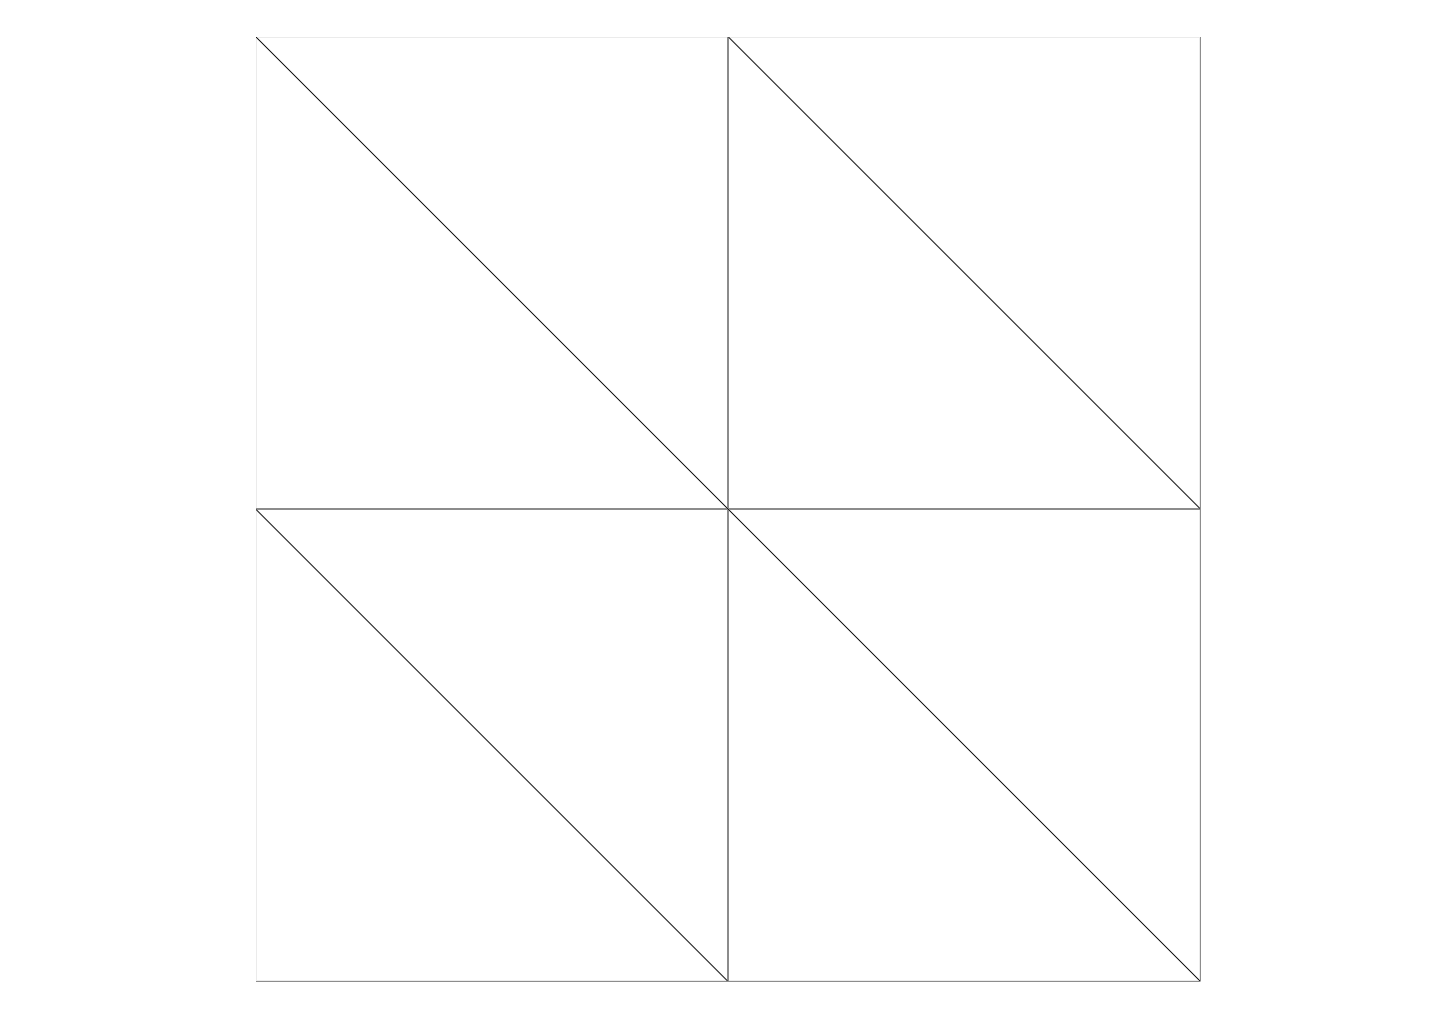
\includegraphics[width=\linewidth]
		{data/synthetic_meshes/square_tesselation_2tri_Dirac_delta_1_v9_f8_wireframe.png}
		\caption{$r=1$, wireframe}\label{fig:sq2.a}
	\end{subfigure}
	\begin{subfigure}[b]{0.32\linewidth}
		
\includegraphics[width=\linewidth]
		{data/synthetic_meshes/square_tesselation_2tri_Dirac_delta_1_v9_f8_funcvals_0iter_crop.png}
		\caption{$r=1$, $c=0$}\label{fig:sq2.b}
	\end{subfigure}
	\begin{subfigure}[b]{0.32\linewidth}
		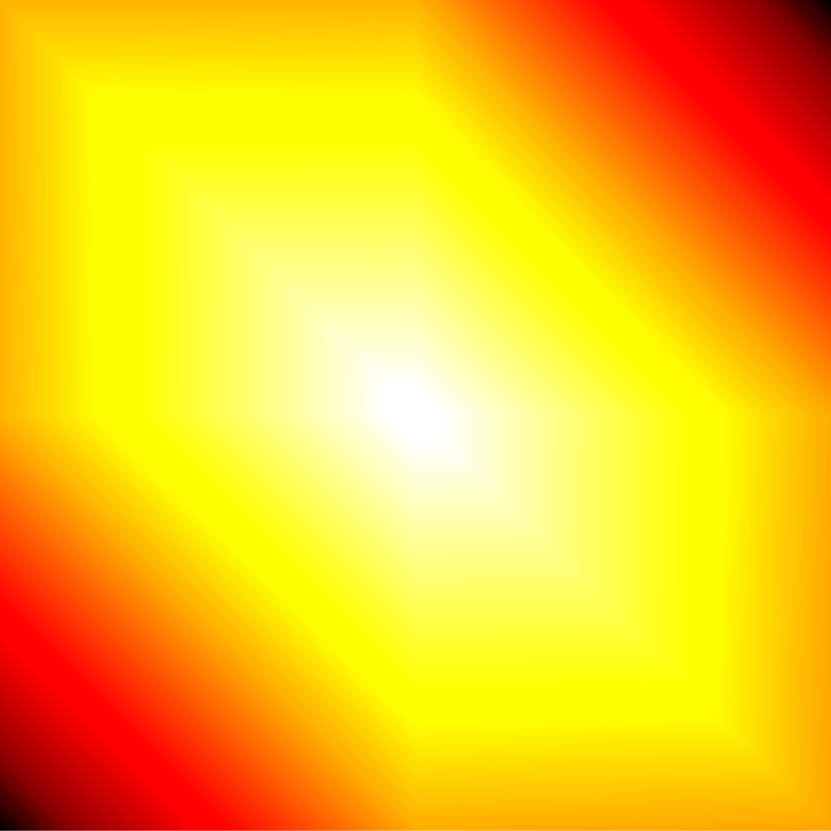
\includegraphics[width=\linewidth]
		{data/synthetic_meshes/square_tesselation_2tri_Dirac_delta_1_v9_f8_funcvals_1iter_crop.png}
		\caption{$r=1$, $c=1$}\label{fig:sq2.c}
	\end{subfigure}

	\bigskip
	\begin{subfigure}[b]{0.32\linewidth}
		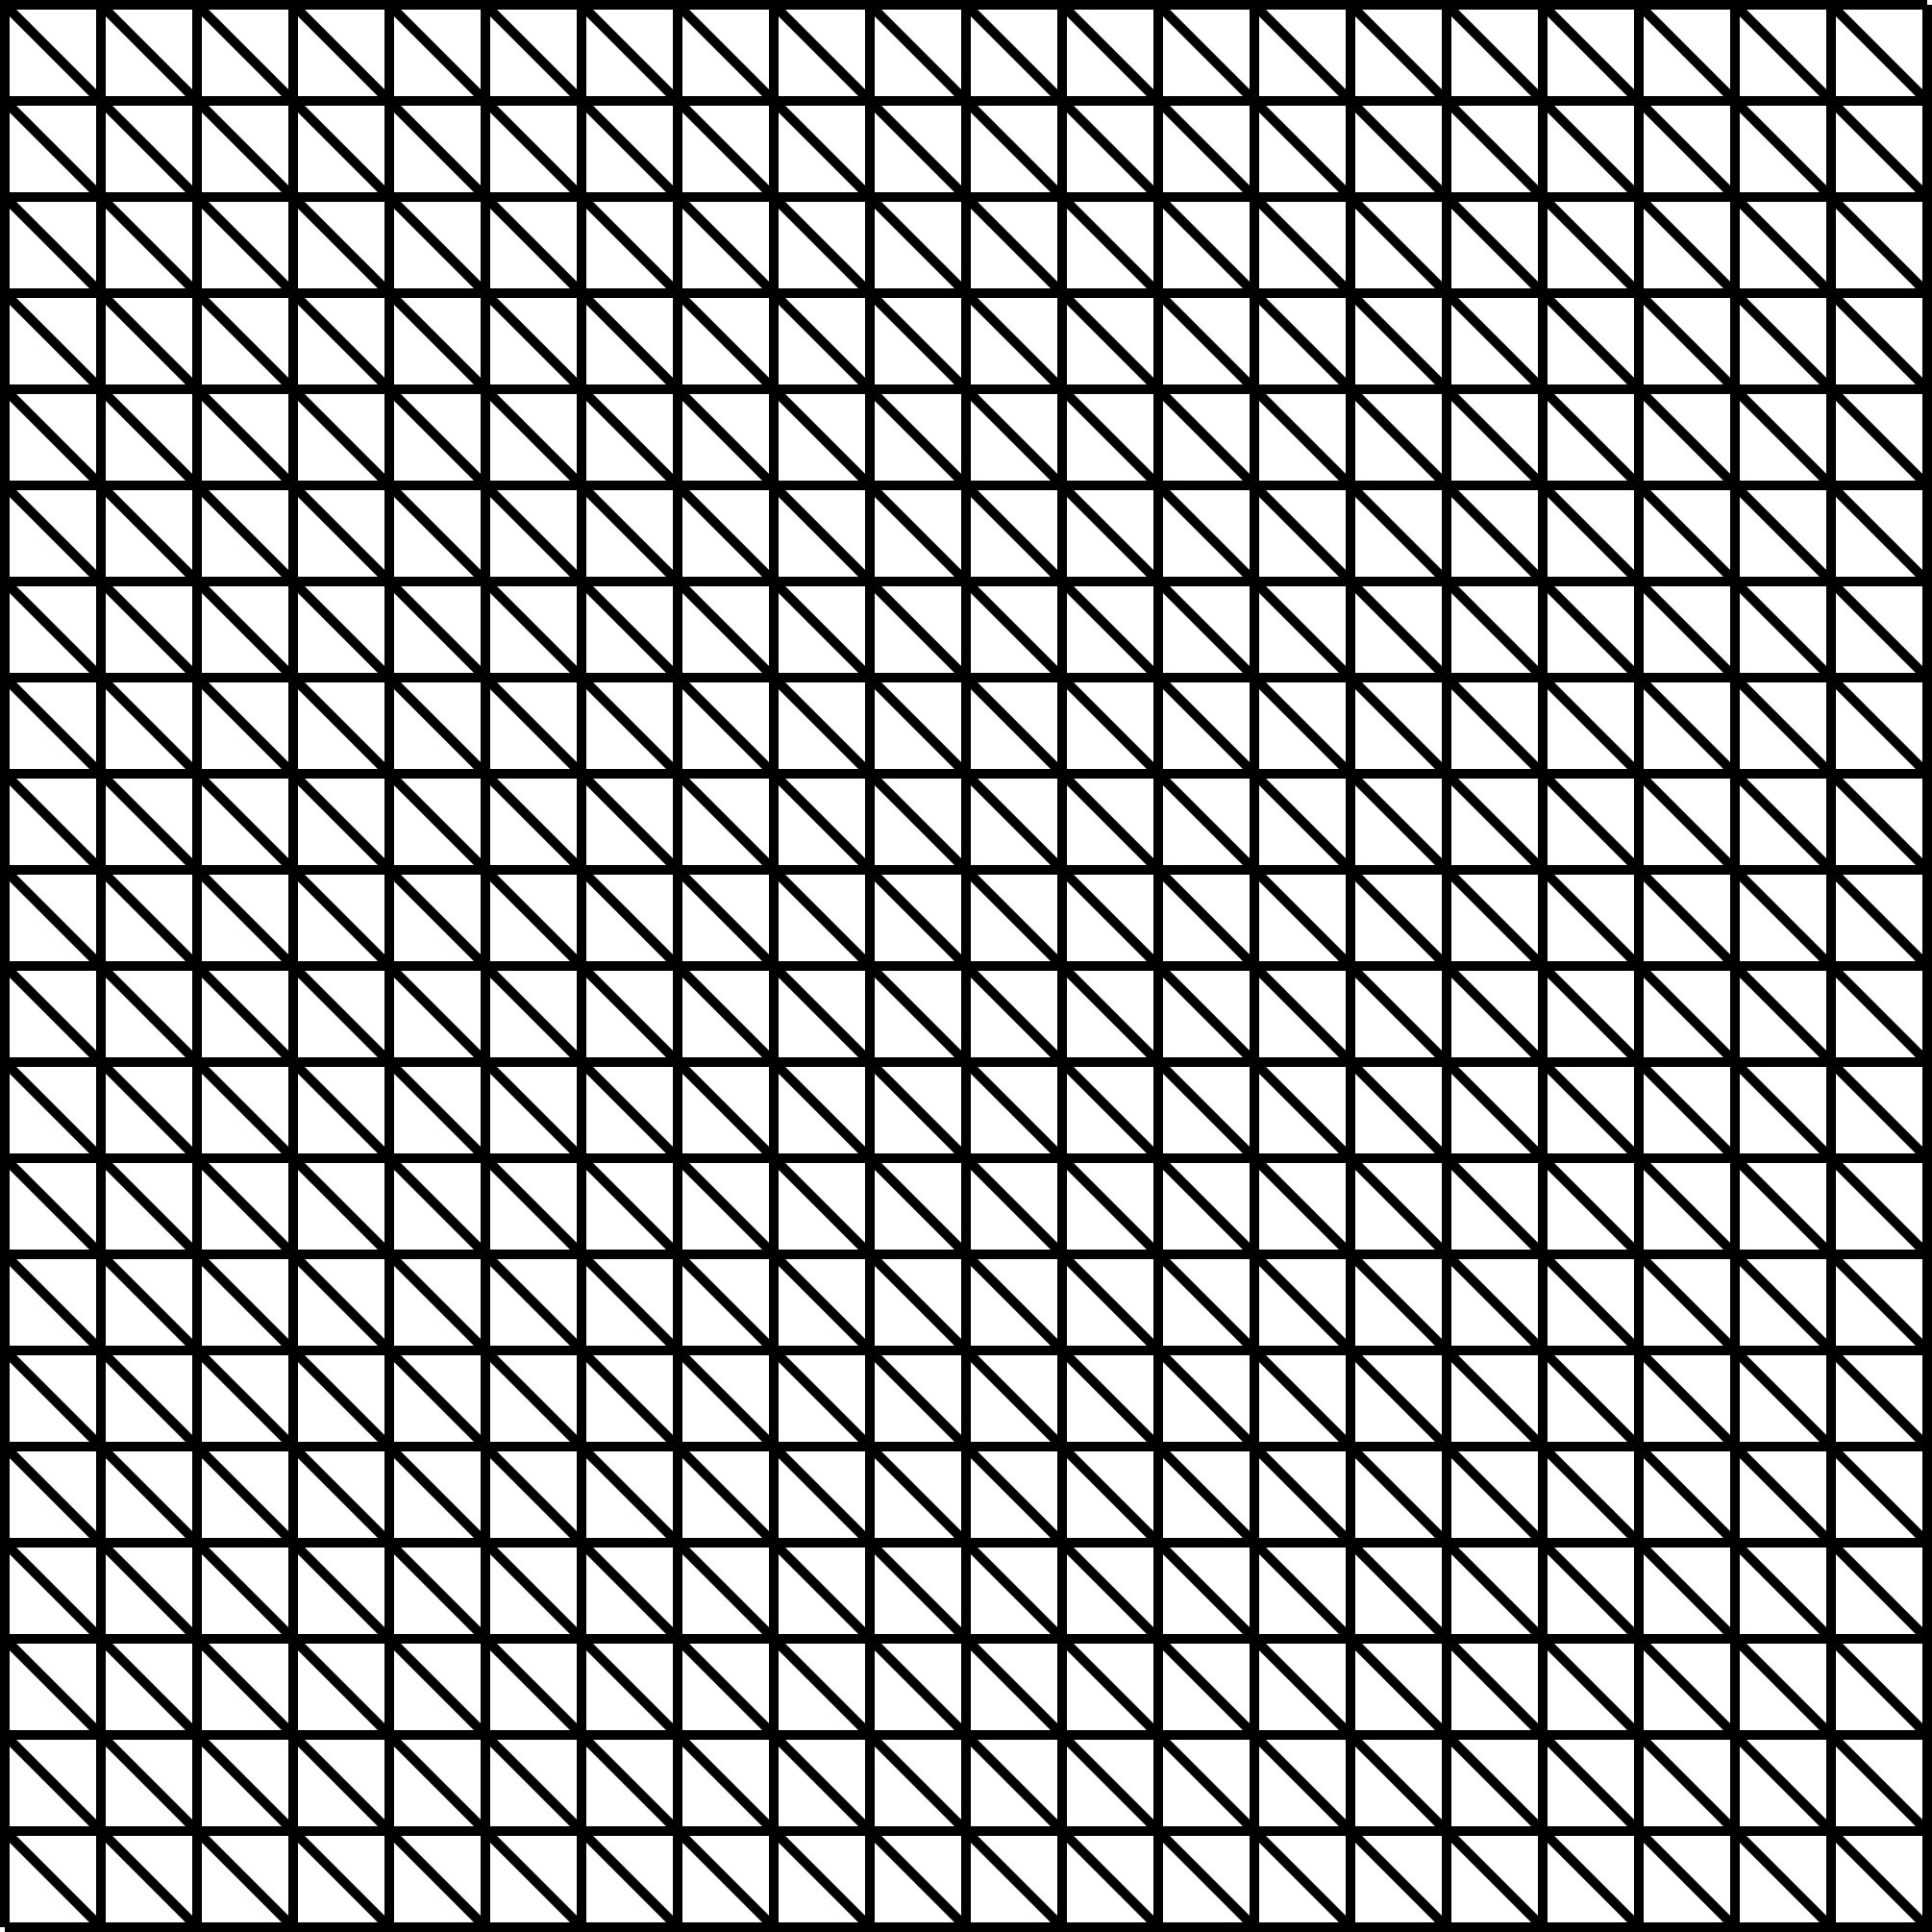
\includegraphics[width=\linewidth]
		{data/synthetic_meshes/square_tesselation_2tri_Dirac_delta_10_v441_f800_wireframe.png}
		\caption{$r=10$, wireframe}\label{fig:sq2.d}
	\end{subfigure}
	\begin{subfigure}[b]{0.32\linewidth}
		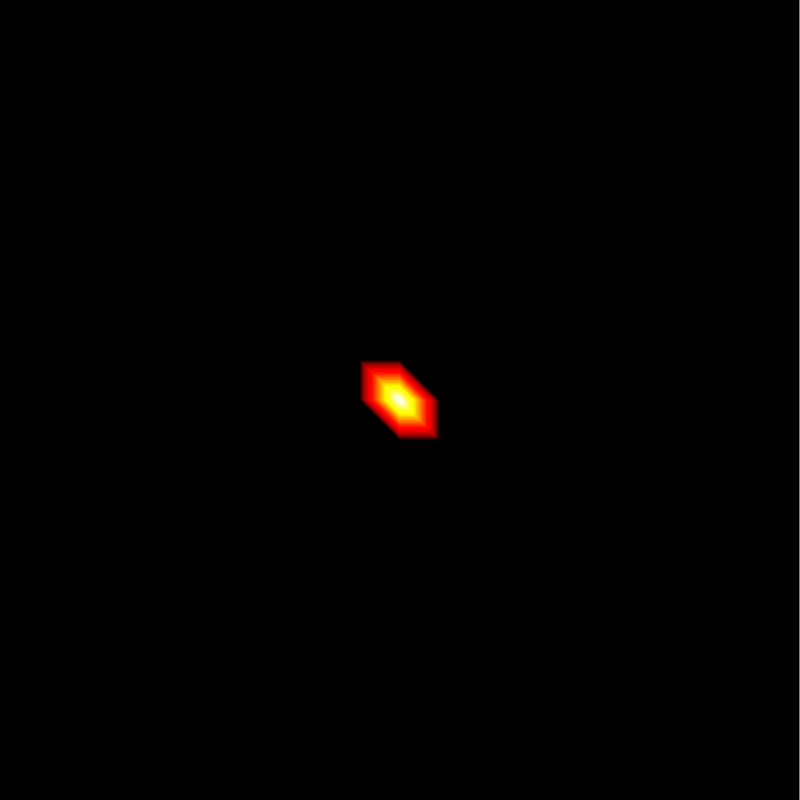
\includegraphics[width=\linewidth]
		{data/synthetic_meshes/square_tesselation_2tri_Dirac_delta_10_v441_f800_funcvals_0iter.png}
		\caption{$r=10$, $c=0$}\label{fig:sq2.e}
	\end{subfigure}
	\begin{subfigure}[b]{0.32\linewidth}
		
\includegraphics[width=\linewidth]
		{data/synthetic_meshes/square_tesselation_2tri_Dirac_delta_10_v441_f800_funcvals_100iter.png}
		\caption{$r=10$, $c=100$}\label{fig:sq2.f}
	\end{subfigure}
\end{figure}

		\end{minipage}
	}
}

%------------------------------------------------
\frame{\frametitle{Quadrisected-Square Tessellations}
	\centering
	\scalebox{0.6}{
		\begin{minipage}{\textwidth}
			\begin{figure}[ht]
	\begin{subfigure}[b]{0.32\linewidth}
		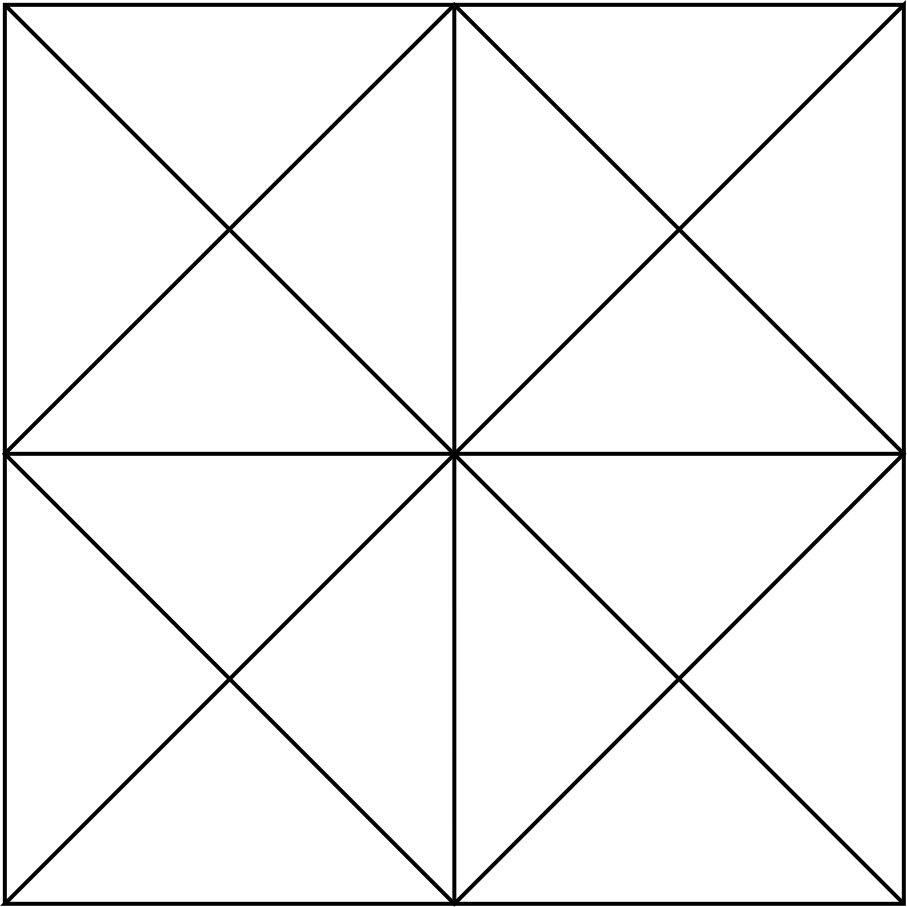
\includegraphics[width=\linewidth]
		{data/synthetic_meshes/square_tesselation_4tri_Dirac_delta_1_v13_f16_wireframe.png}
		\caption{$r=1$, wireframe}\label{fig:sq2.a}
	\end{subfigure}
	\begin{subfigure}[b]{0.32\linewidth}
		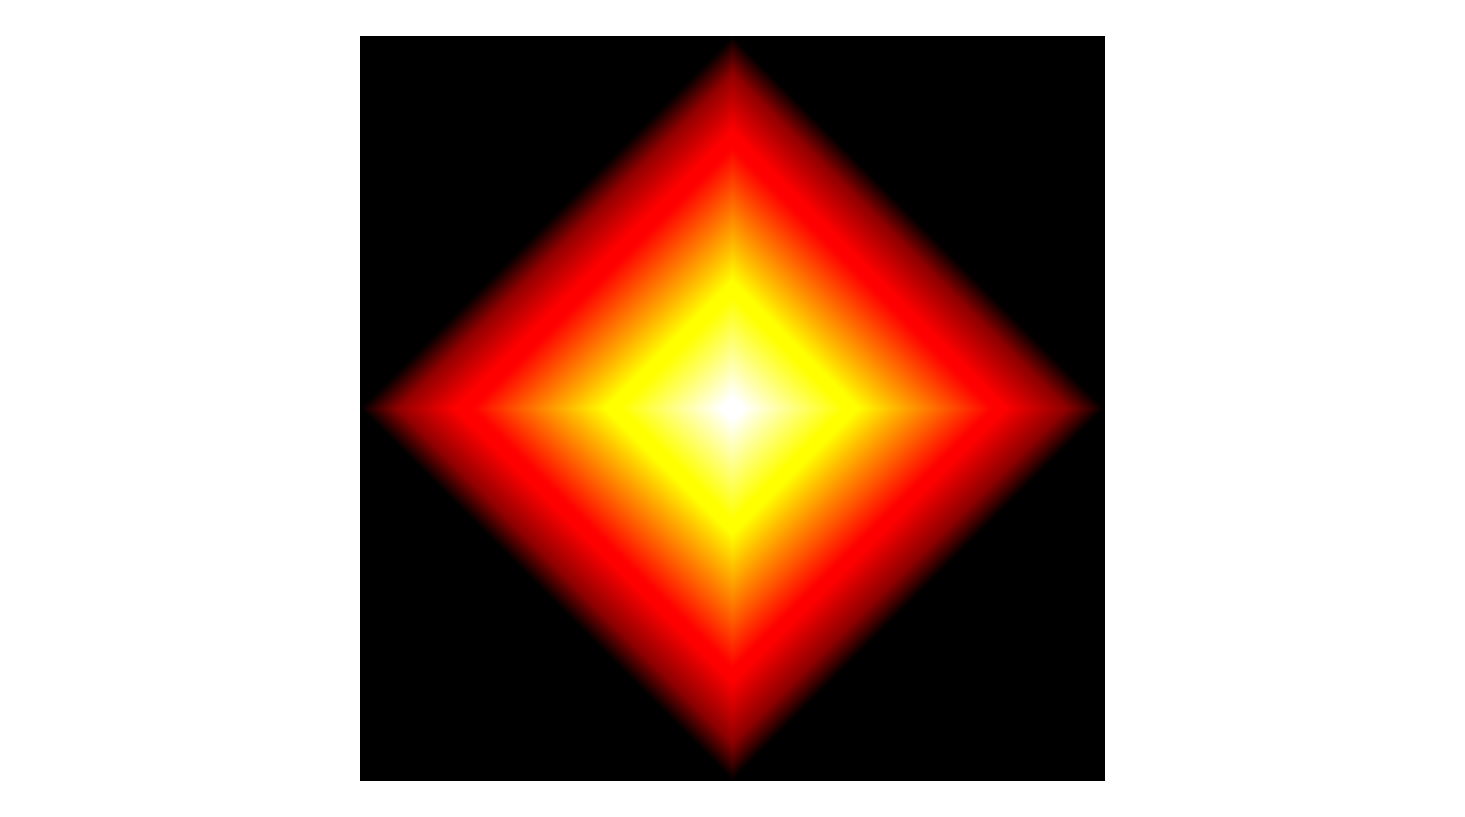
\includegraphics[width=\linewidth]
		{data/synthetic_meshes/square_tesselation_4tri_Dirac_delta_1_v13_f16_funcvals_0iter.png}
		\caption{$r=1$, $c=0$}\label{fig:sq2.b}
	\end{subfigure}
	\begin{subfigure}[b]{0.32\linewidth}
		
\includegraphics[width=\linewidth]
		{data/synthetic_meshes/square_tesselation_4tri_Dirac_delta_1_v13_f16_funcvals_1iter.png}
		\caption{$r=1$, $c=1$}\label{fig:sq2.c}
	\end{subfigure}

	\bigskip
	\begin{subfigure}[b]{0.32\linewidth}
		
\includegraphics[width=\linewidth]
		{data/synthetic_meshes/square_tesselation_4tri_Dirac_delta_10_v841_f1600_wireframe_2.png}
		\caption{$r=10$, wireframe}\label{fig:sq2.d}
	\end{subfigure}
	\begin{subfigure}[b]{0.32\linewidth}
		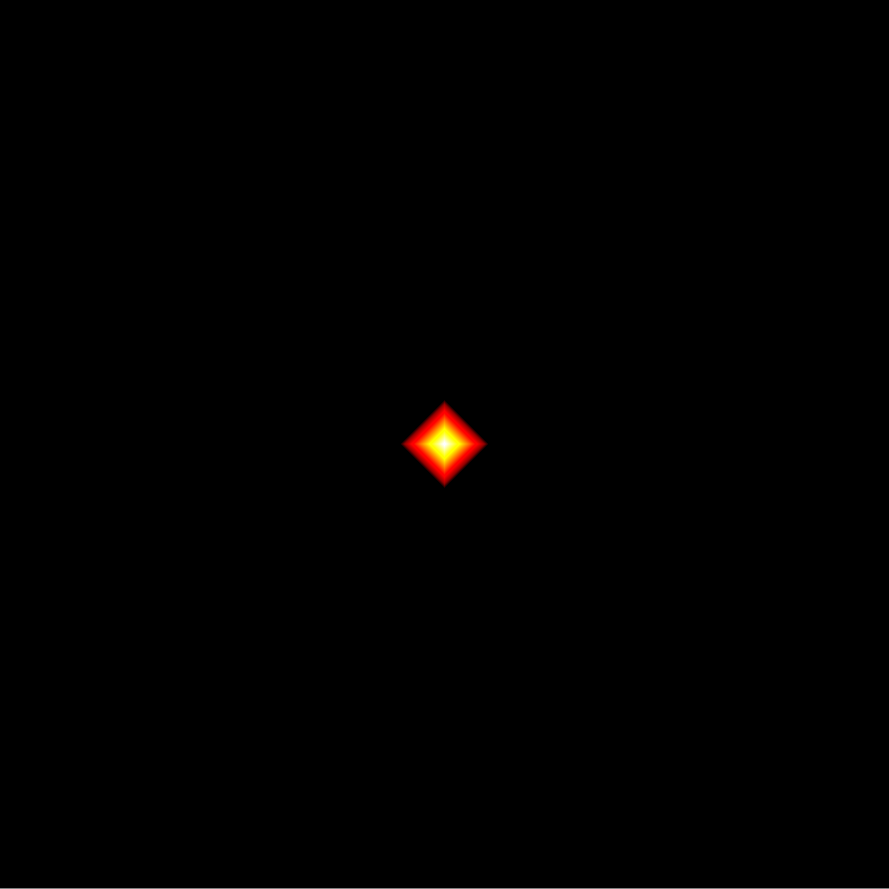
\includegraphics[width=\linewidth]
		{data/synthetic_meshes/square_tesselation_4tri_Dirac_delta_10_v841_f1600_funcvals_0iter.png}
		\caption{$r=10$, $c=0$}\label{fig:sq2.e}
	\end{subfigure}
	\begin{subfigure}[b]{0.32\linewidth}
		
\includegraphics[width=\linewidth]
		{data/synthetic_meshes/square_tesselation_4tri_Dirac_delta_10_v841_f1600_funcvals_100iter.png}
		\caption{$r=10$, $c=100$}\label{fig:sq2.f}
	\end{subfigure}
\end{figure}

		\end{minipage}
	}
}

%------------------------------------------------
\frame{\frametitle{Hexagonal Tessellations}
	\centering
	\scalebox{0.6}{
		\begin{minipage}{\textwidth}
			\begin{figure}[ht]
	\begin{subfigure}[b]{0.32\linewidth}
		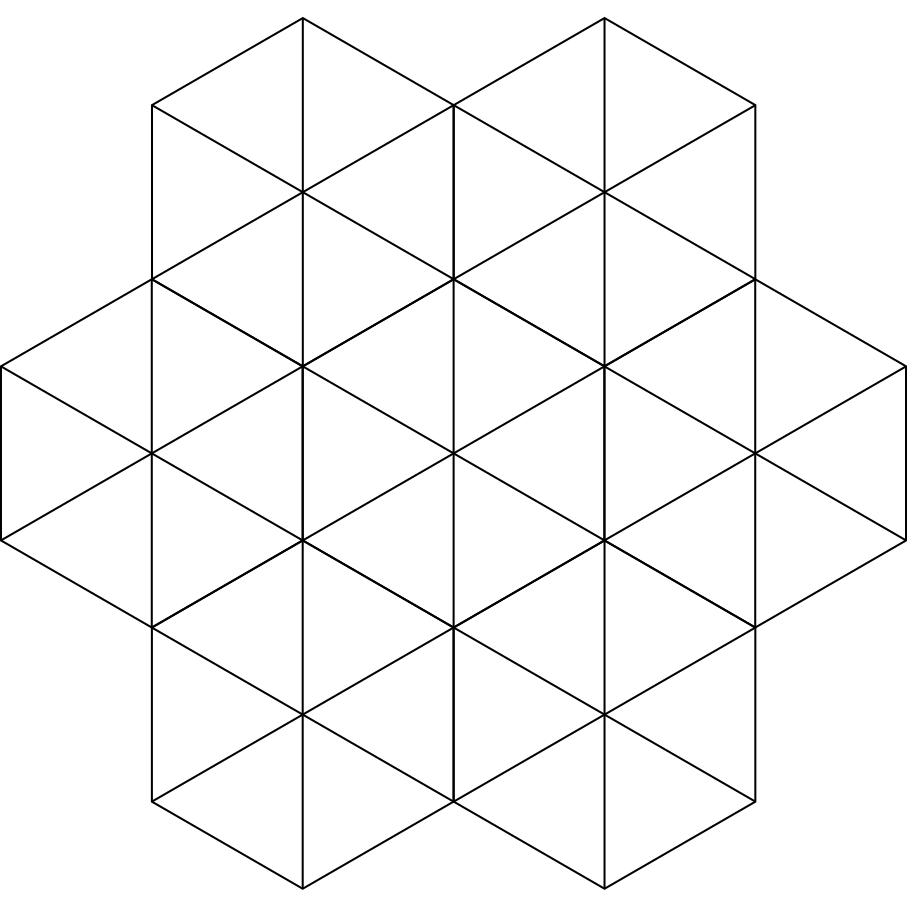
\includegraphics[width=\linewidth]
		{data/synthetic_meshes/hexagonal_tessellation_Dirac_delta_1_v31_f42_wireframe.png}
		\caption{$r=1$, wireframe}\label{fig:hex.a}
	\end{subfigure}
	\begin{subfigure}[b]{0.32\linewidth}
		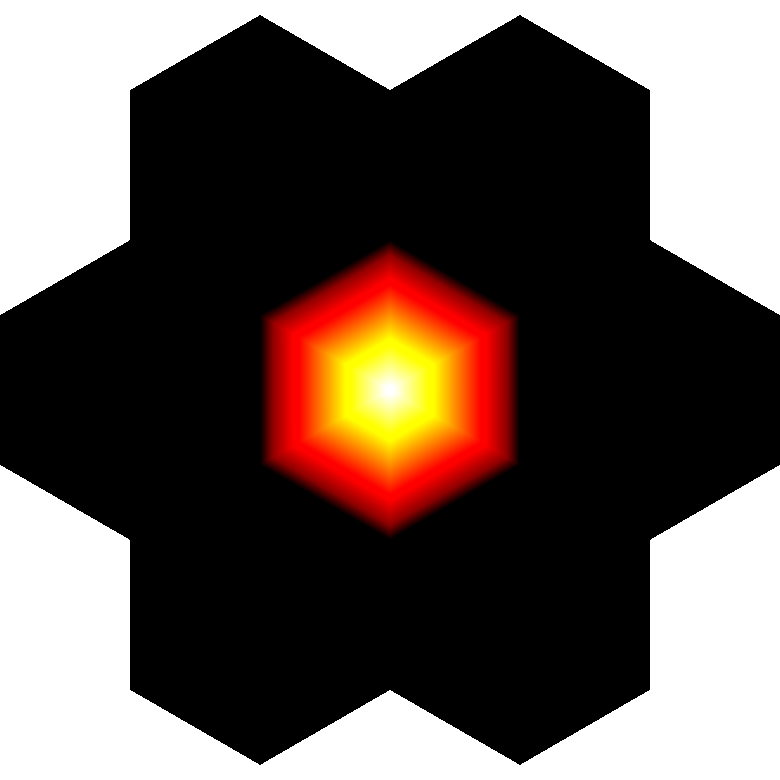
\includegraphics[width=\linewidth]
		{data/synthetic_meshes/hexagonal_tessellation_Dirac_delta_1_v31_f42_funcvals_0iter_crop.png}
		\caption{$r=1$, $c=0$}\label{fig:hex.b}
	\end{subfigure}
	\begin{subfigure}[b]{0.32\linewidth}
		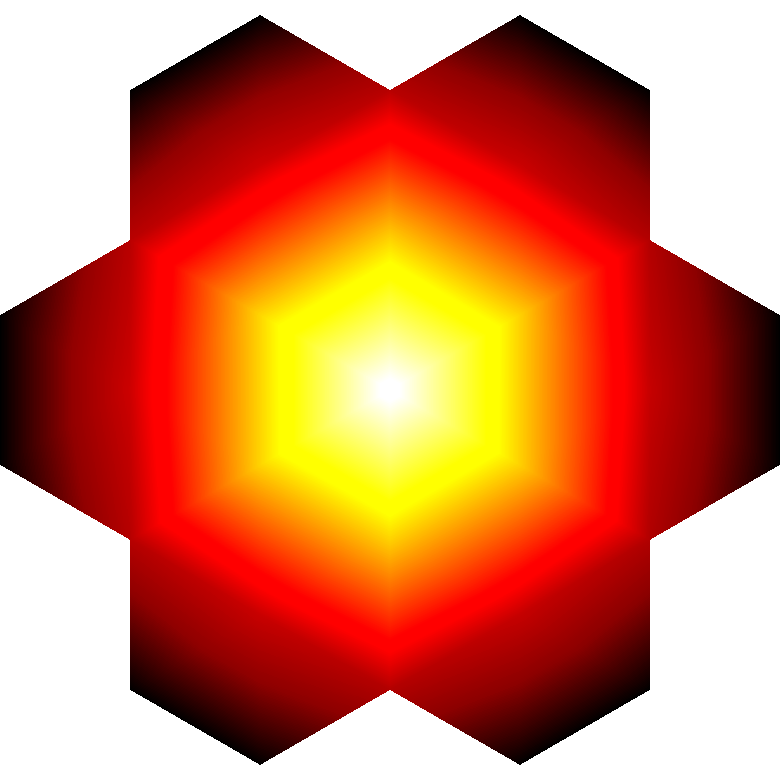
\includegraphics[width=\linewidth]
		{data/synthetic_meshes/hexagonal_tessellation_Dirac_delta_1_v31_f42_funcvals_2iter_crop.png}
		\caption{$r=1$, $c=2$}\label{fig:hex.c}
	\end{subfigure}

	\begin{subfigure}[b]{0.32\linewidth}
		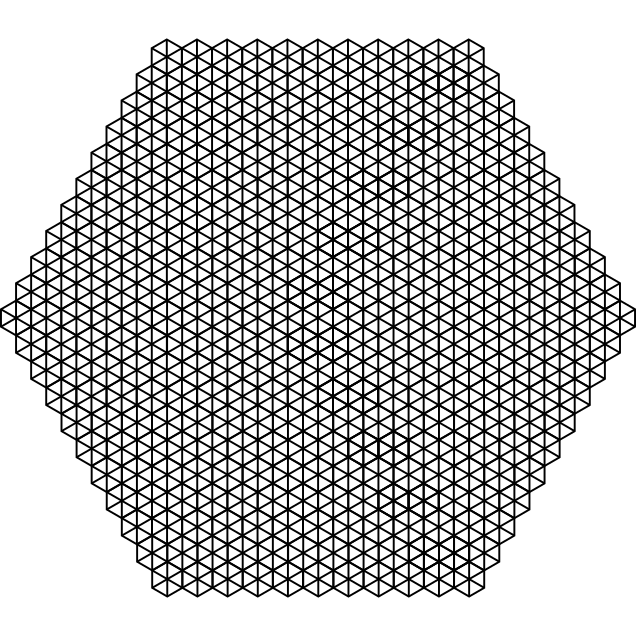
\includegraphics[width=\linewidth]
		{data/synthetic_meshes/hexagonal_tessellation_Dirac_delta_10_v1057_f1986_wireframe.png}
		\caption{$r=10$, wireframe}\label{fig:hex.d}
	\end{subfigure}
	\begin{subfigure}[b]{0.32\linewidth}
		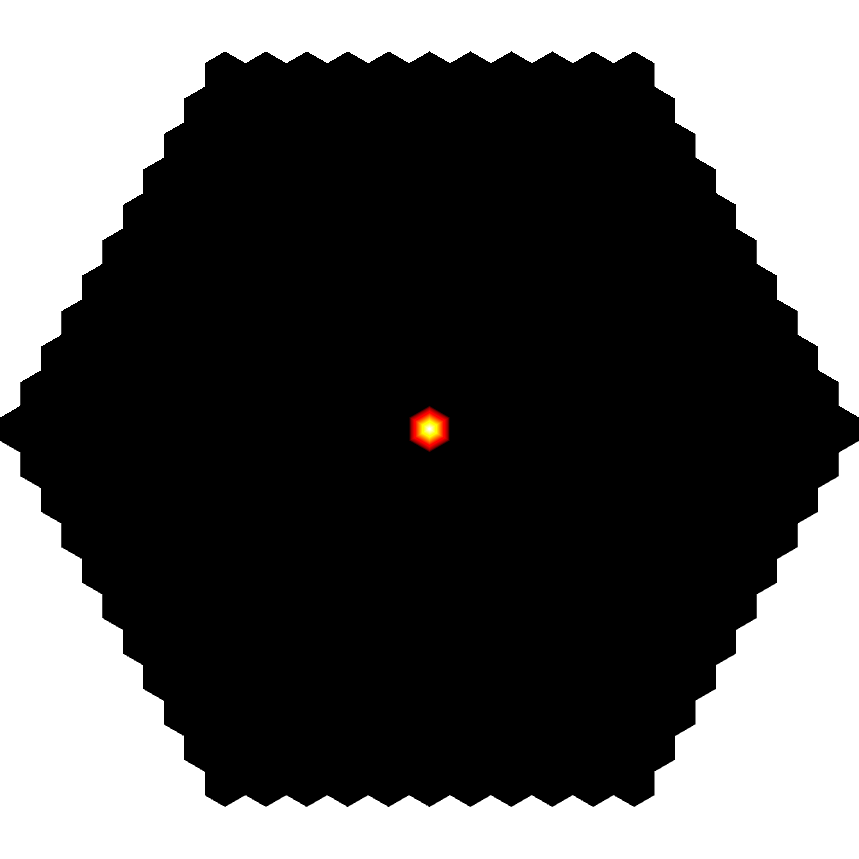
\includegraphics[width=\linewidth]
		{data/synthetic_meshes/hexagonal_tessellation_Dirac_delta_10_v1057_f1986_funcvals_0iter_crop.png}
		\caption{$r=10$, $c=0$}\label{fig:hex.e}
	\end{subfigure}
	\begin{subfigure}[b]{0.32\linewidth}
		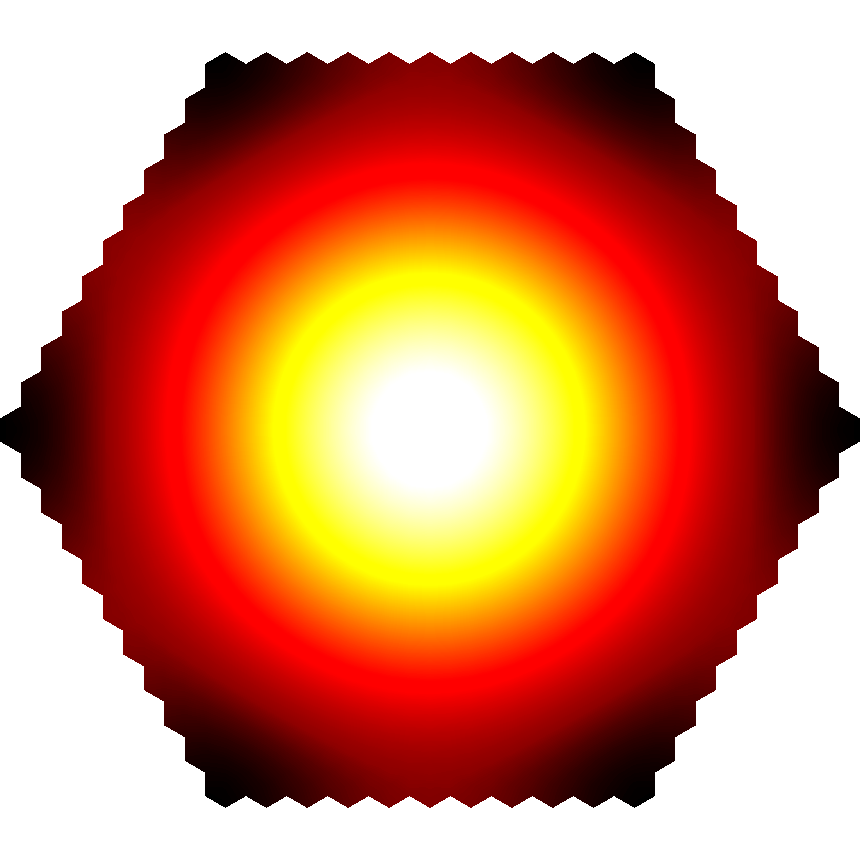
\includegraphics[width=\linewidth]
		{data/synthetic_meshes/hexagonal_tessellation_Dirac_delta_10_v1057_f1986_funcvals_200iter_crop.png}
		\caption{$r=10$, $c=200$}\label{fig:hex.f}
	\end{subfigure}
\end{figure}

		\end{minipage}
	}
}

%------------------------------------------------
\frame{\frametitle{Random Triangulated Discs}
	\centering
	\scalebox{0.6}{
		\begin{minipage}{\textwidth}
			\begin{figure}[ht]
	\begin{subfigure}[b]{0.32\linewidth}
		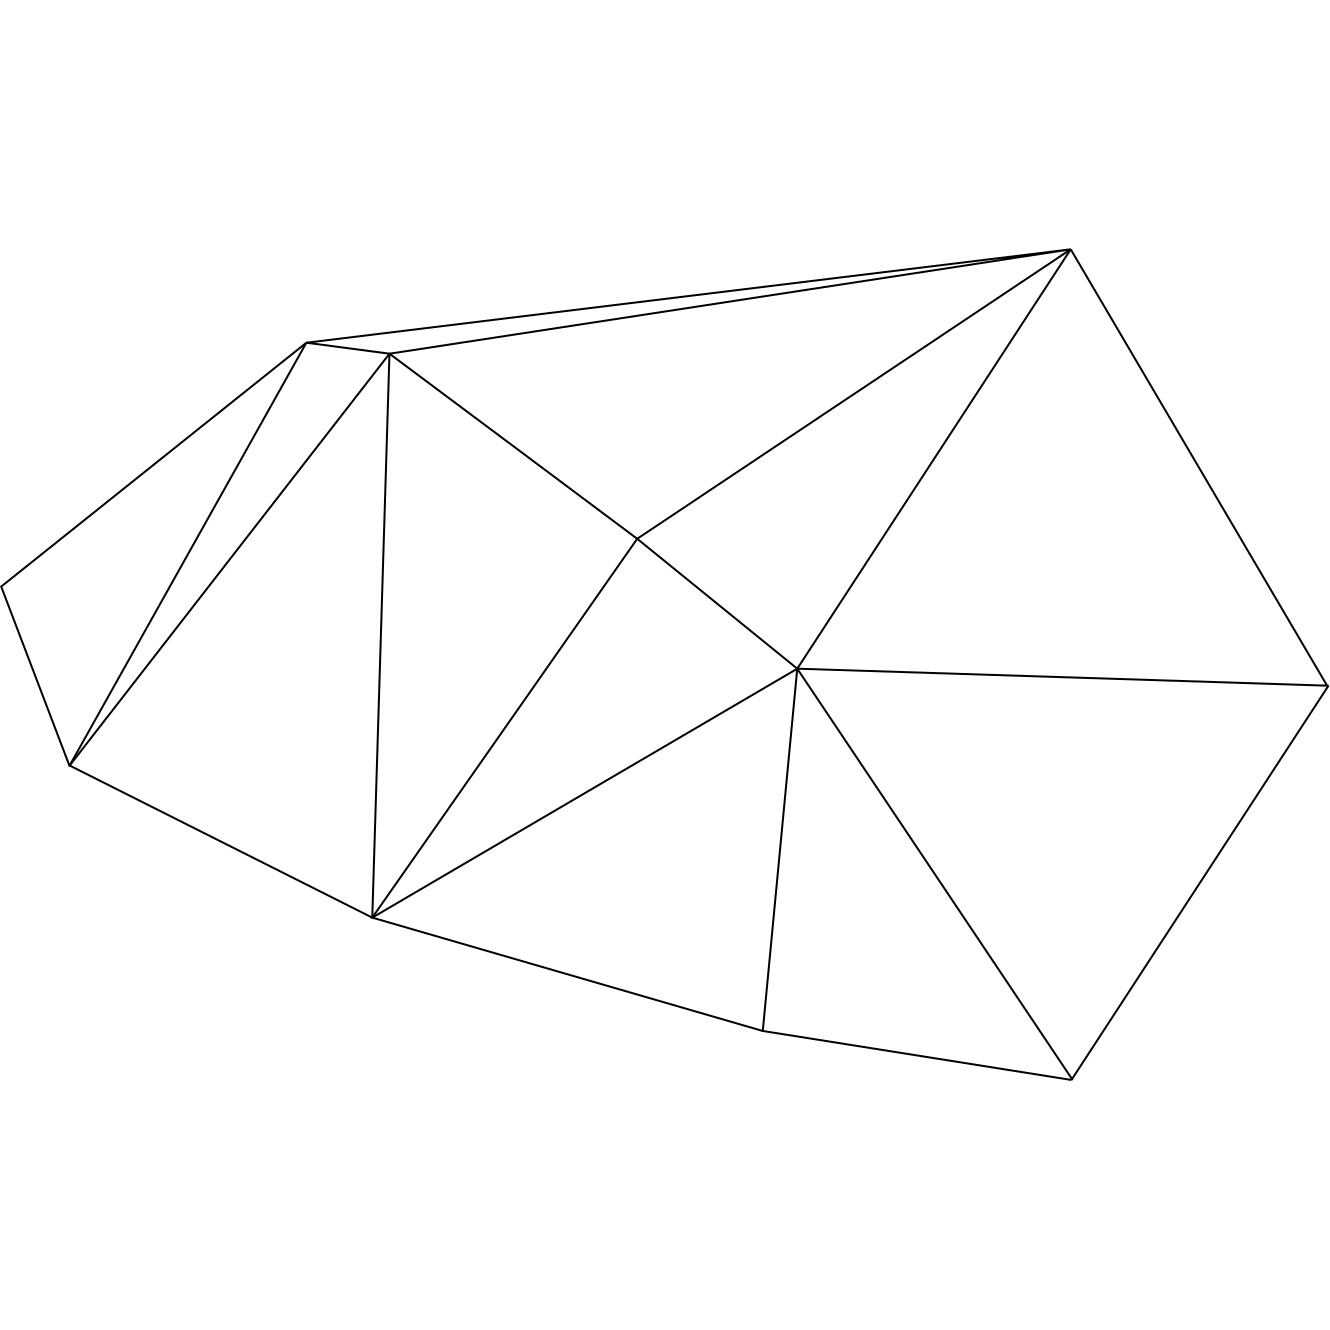
\includegraphics[width=\linewidth]
		{data/synthetic_meshes/random_circle_tessellation_Dirac_delta_1_v11_f12_wireframe.png}
		\caption{$r=1$, $p=11$, wireframe}\label{fig:rcirc.a}
	\end{subfigure}
	\begin{subfigure}[b]{0.32\linewidth}
		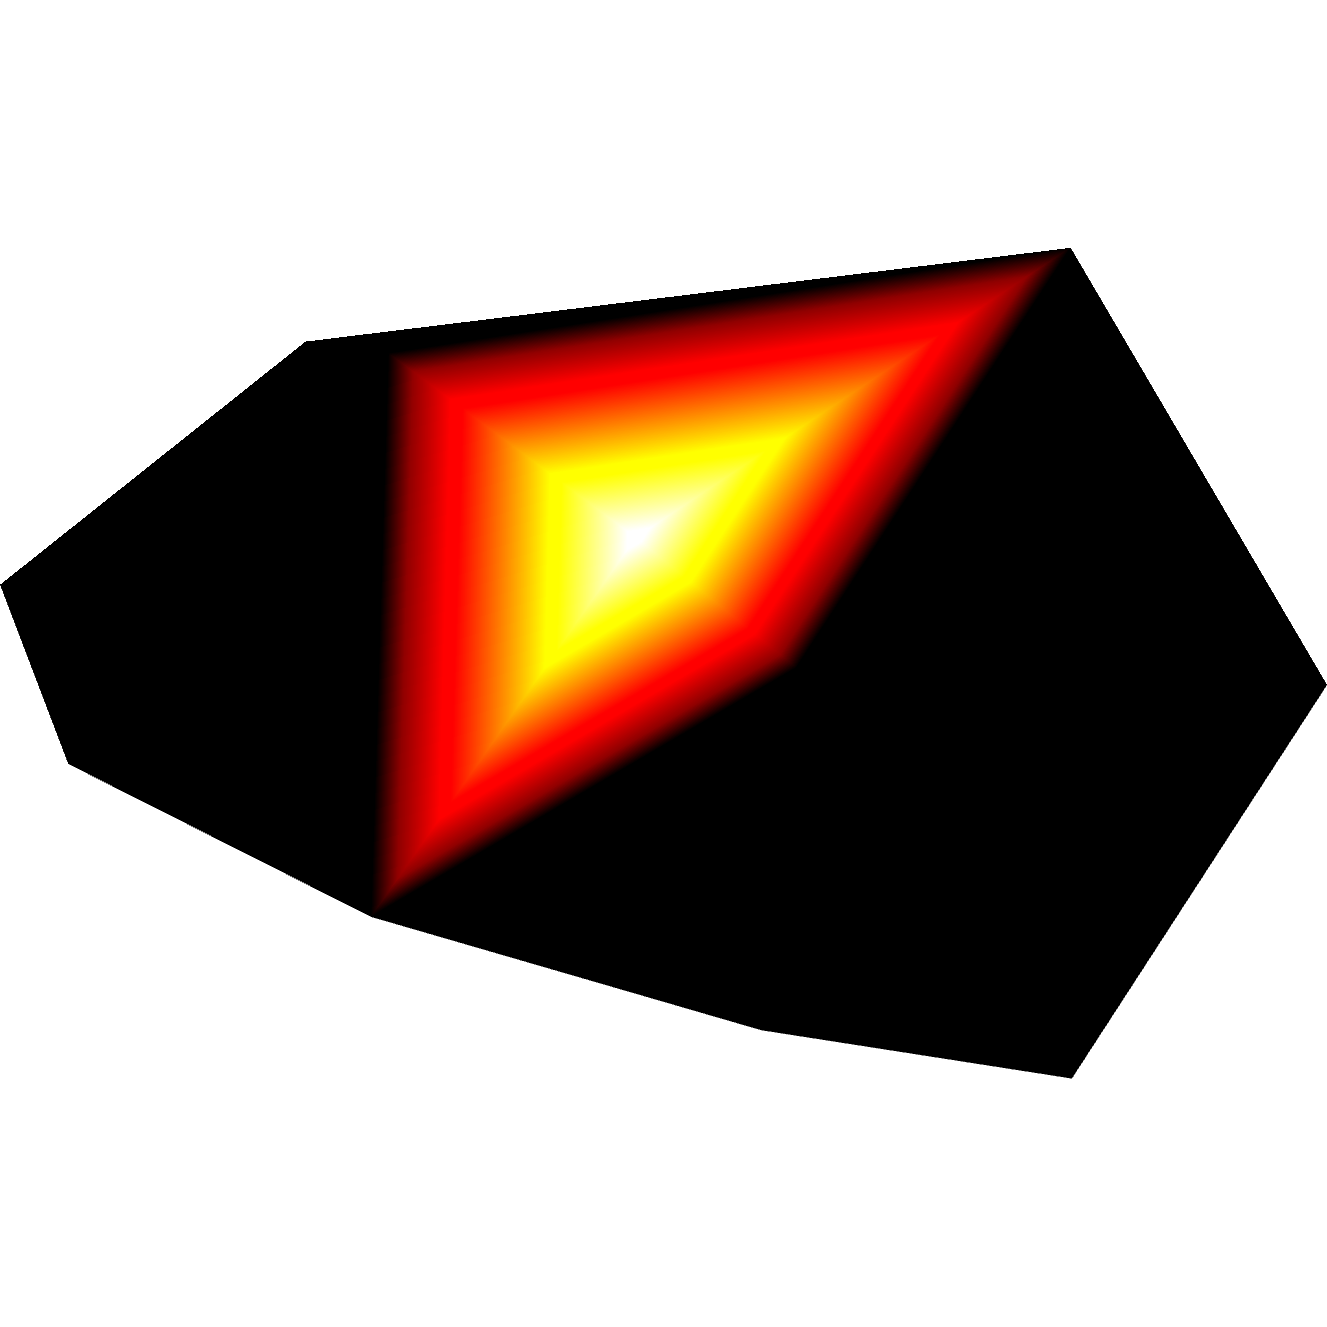
\includegraphics[width=\linewidth]
		{data/synthetic_meshes/random_circle_tessellation_Dirac_delta_1_v11_f12_funcvals_0iter.png}
		\caption{$r=1$, $p=11$, $c=0$}\label{fig:rcirc.c}
	\end{subfigure}
	\begin{subfigure}[b]{0.32\linewidth}
		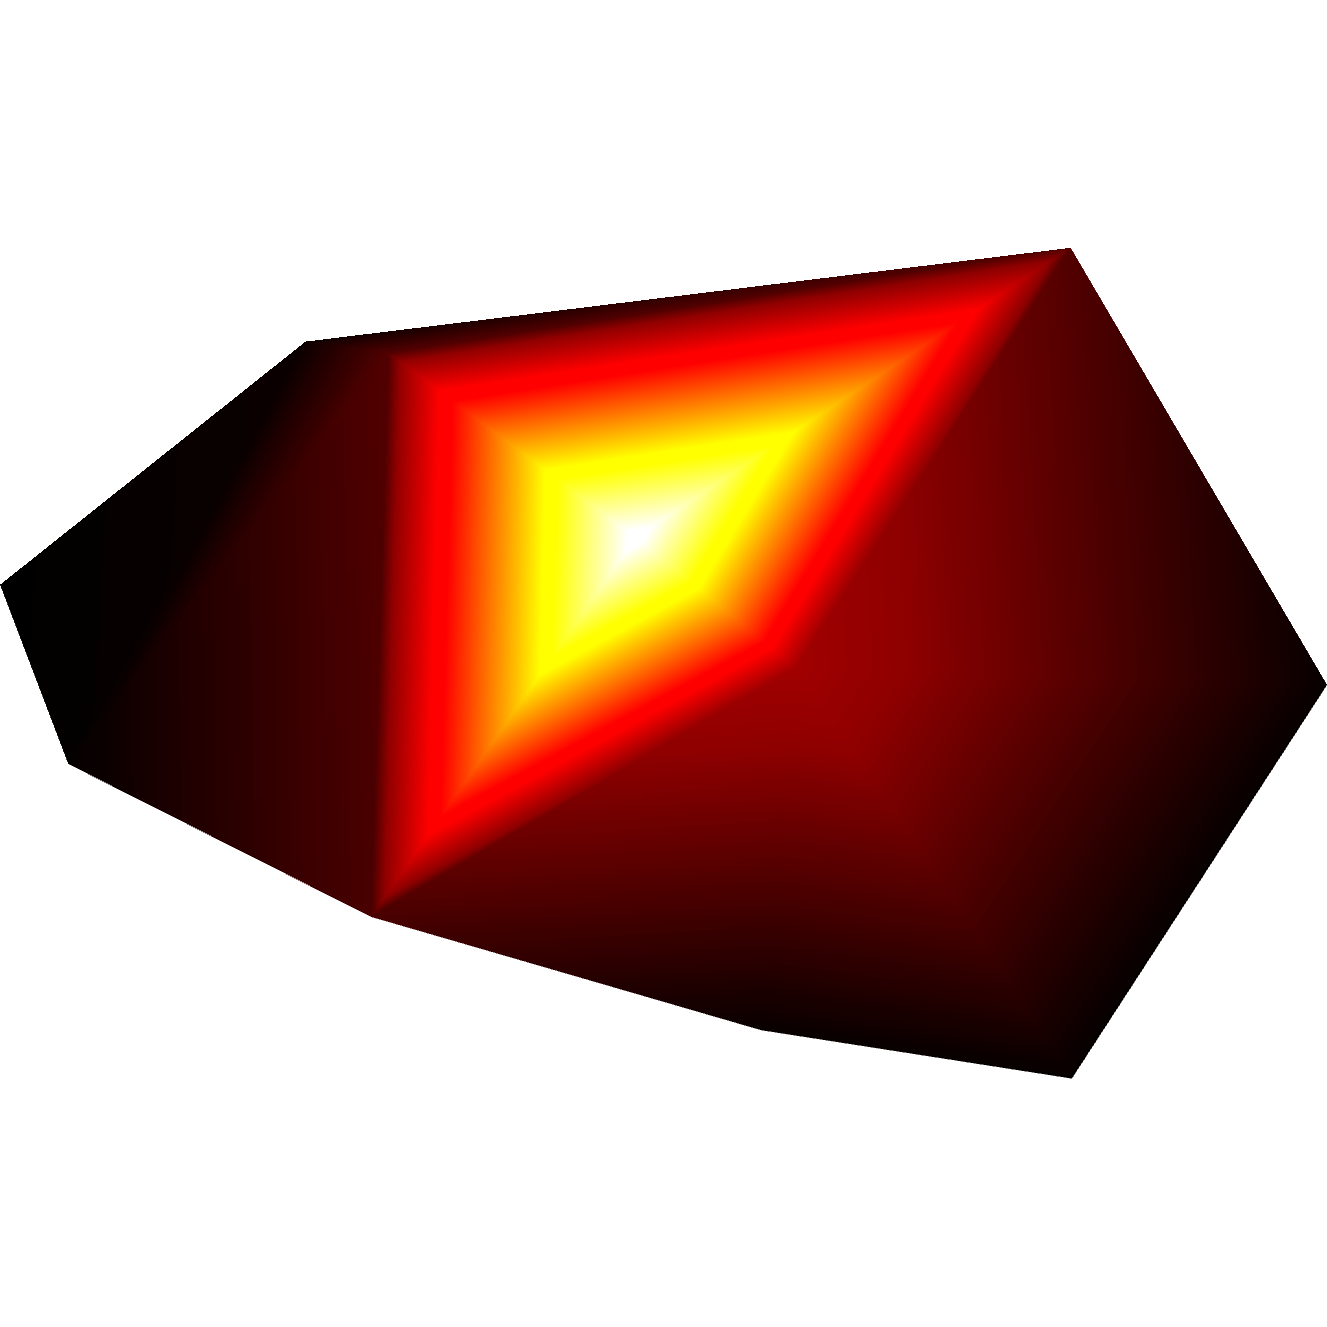
\includegraphics[width=\linewidth,]
		{data/synthetic_meshes/random_circle_tessellation_Dirac_delta_1_v11_f12_funcvals_2iter.png}
		\caption{$r=1$, $p=11$, $c=2$}\label{fig:rcirc.e}
	\end{subfigure}

	\bigskip
	\begin{subfigure}[b]{0.32\linewidth}
		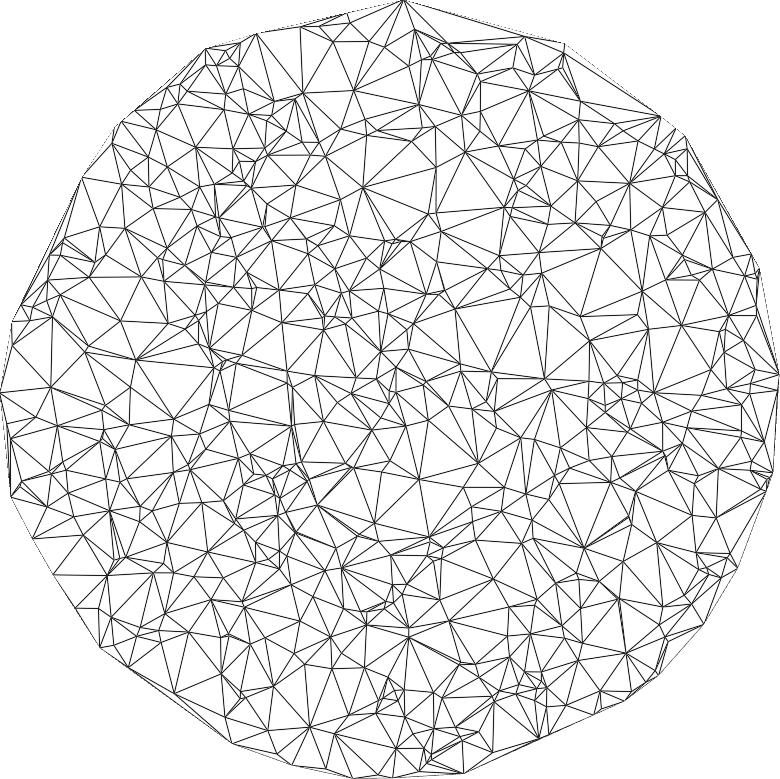
\includegraphics[width=\linewidth]
		{data/synthetic_meshes/random_circle_tessellation_Dirac_delta_10_v641_f1252_wireframe.png}
		\caption{$r=10$, $p=641$, wireframe}\label{fig:rcirc.b}
	\end{subfigure}
	\begin{subfigure}[b]{0.32\linewidth}
		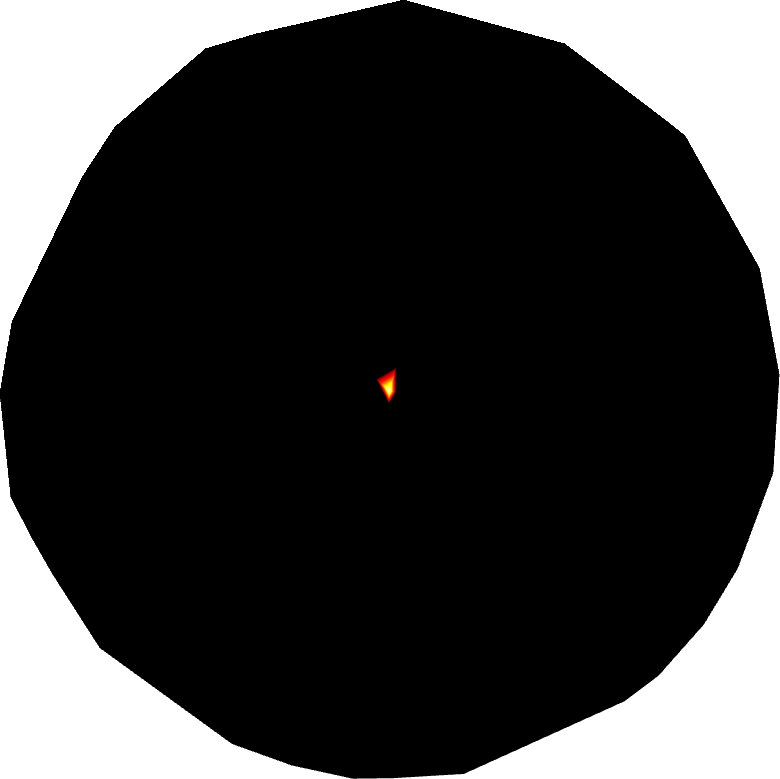
\includegraphics[width=\linewidth]
		{data/synthetic_meshes/random_circle_tessellation_Dirac_delta_10_v641_f1252_funcvals_0iter.png}
		\caption{$r=10$, $p=641$, $c=0$}\label{fig:rcirc.d}
	\end{subfigure}
	\begin{subfigure}[b]{0.32\linewidth}
		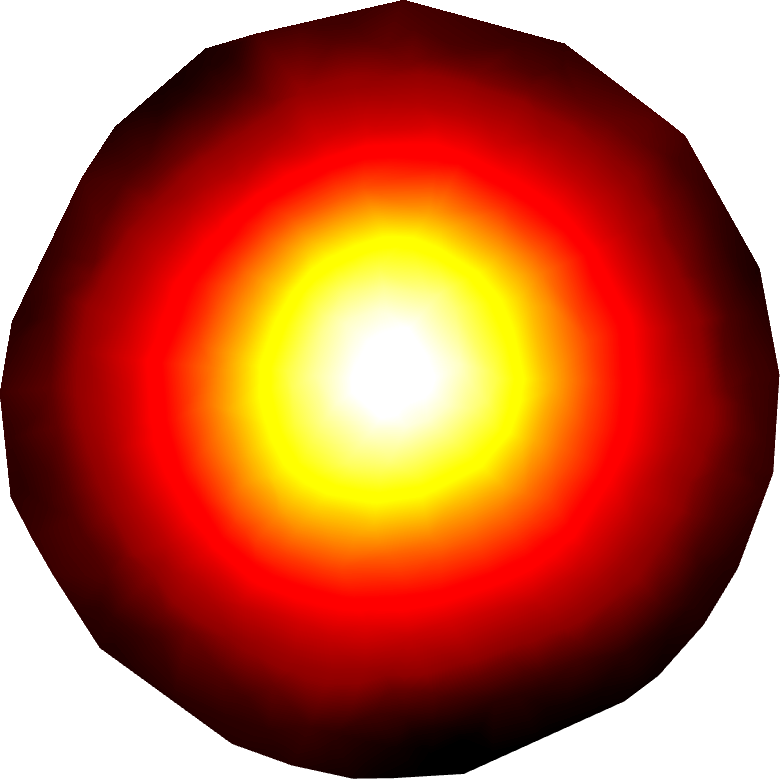
\includegraphics[width=\linewidth]
		{data/synthetic_meshes/random_circle_tessellation_Dirac_delta_10_v641_f1252_funcvals_10000iter.png}
		\caption{$r=10$, $p=641$, $c=10^4$}\label{fig:rcirc.f}
	\end{subfigure}
\end{figure}


		\end{minipage}
	}
}


%================================================
\subsection{Filter Response On Acquired Data}

%------------------------------------------------
\frame{\frametitle{The University of Heidelberg Seal}
	\vspace*{1cm}
	\centering
	\scalebox{1.0}{
		\begin{minipage}{\textwidth}
			\begin{figure}[ht]
	\begin{subfigure}[b]{0.32\linewidth}
		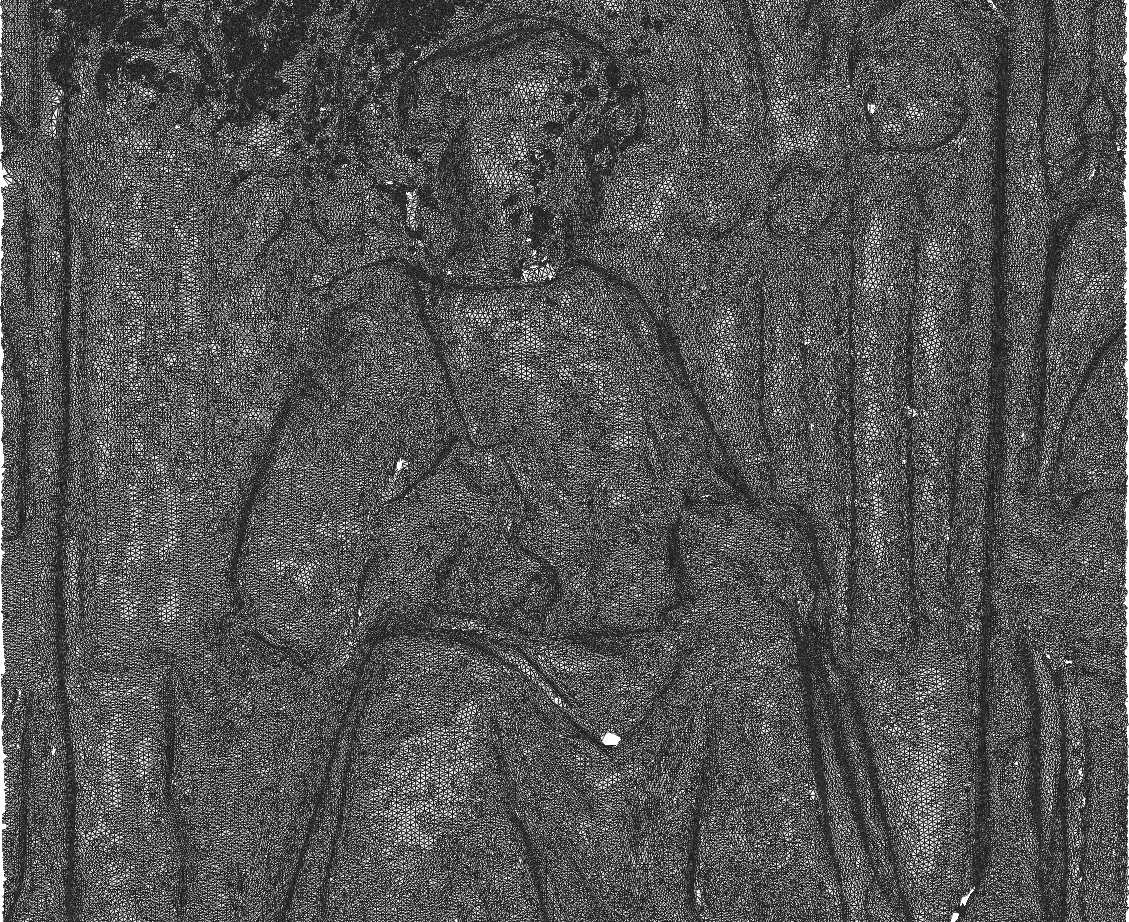
\includegraphics[width=\linewidth]{data/acquired_meshes/unisiegel_wireframe.png}
		\caption{wireframe}\label{fig:unisiegel.a}
	\end{subfigure}
	\begin{subfigure}[b]{0.32\linewidth}
		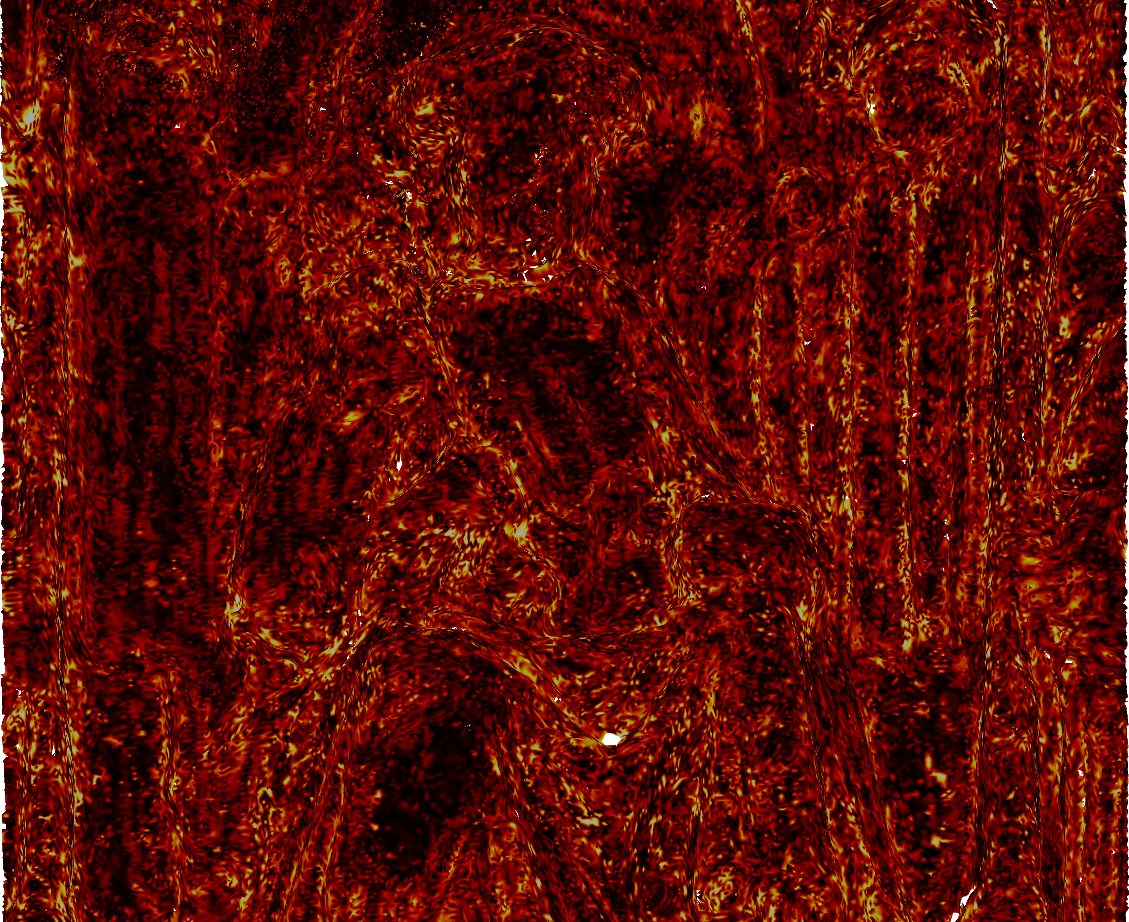
\includegraphics[width=\linewidth]{data/acquired_meshes/unisiegel_0iter.png}
		\caption{$c=0$}\label{fig:unisiegel.b}
	\end{subfigure}
	\begin{subfigure}[b]{0.32\linewidth}
		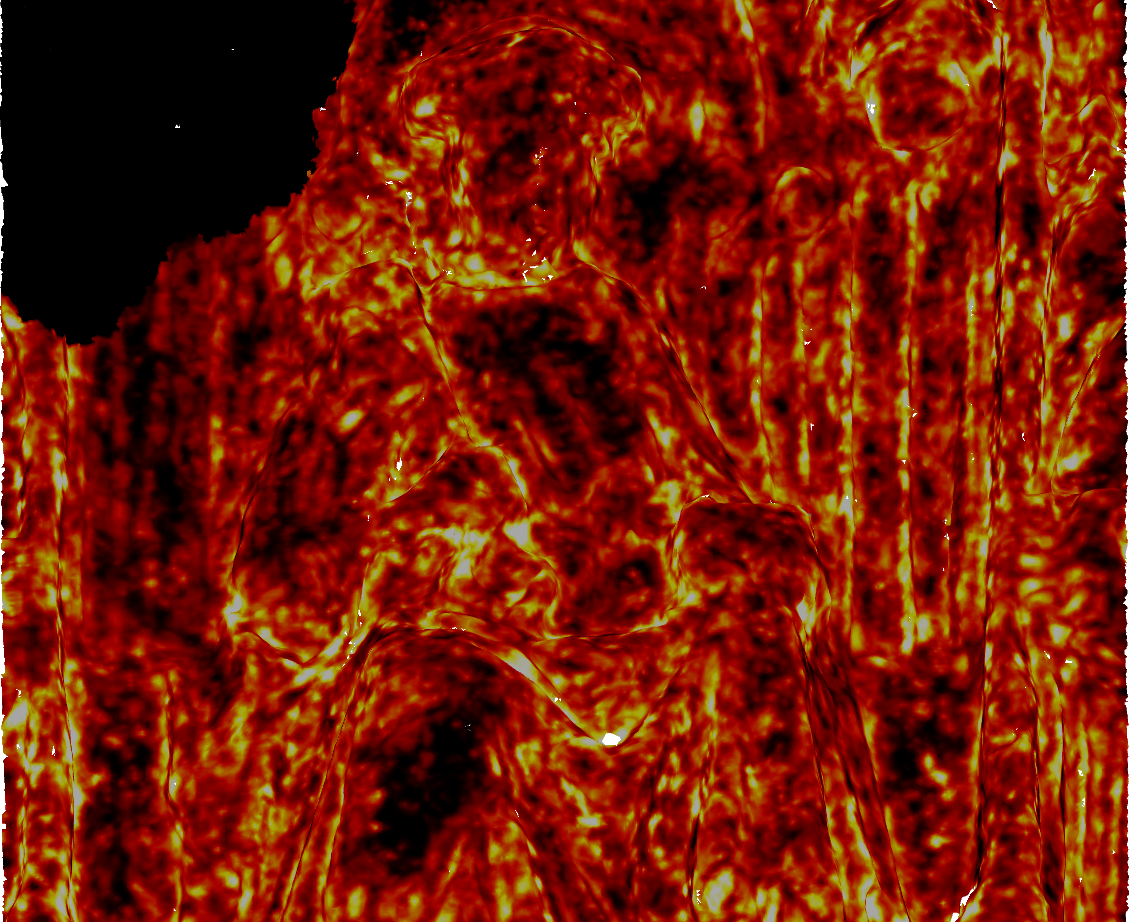
\includegraphics[width=\linewidth]{data/acquired_meshes/unisiegel_100iter.png}
		\caption{$c=100$}\label{fig:unisiegel.c}
	\end{subfigure}
\end{figure}

		\end{minipage}
	}
}

%------------------------------------------------
\frame{\frametitle{A flat surface from ILATO}
	\centering
	\scalebox{0.70}{
		\begin{minipage}{\textwidth}
			\begin{figure}[ht]
	\begin{subfigure}[b]{0.49\linewidth}
		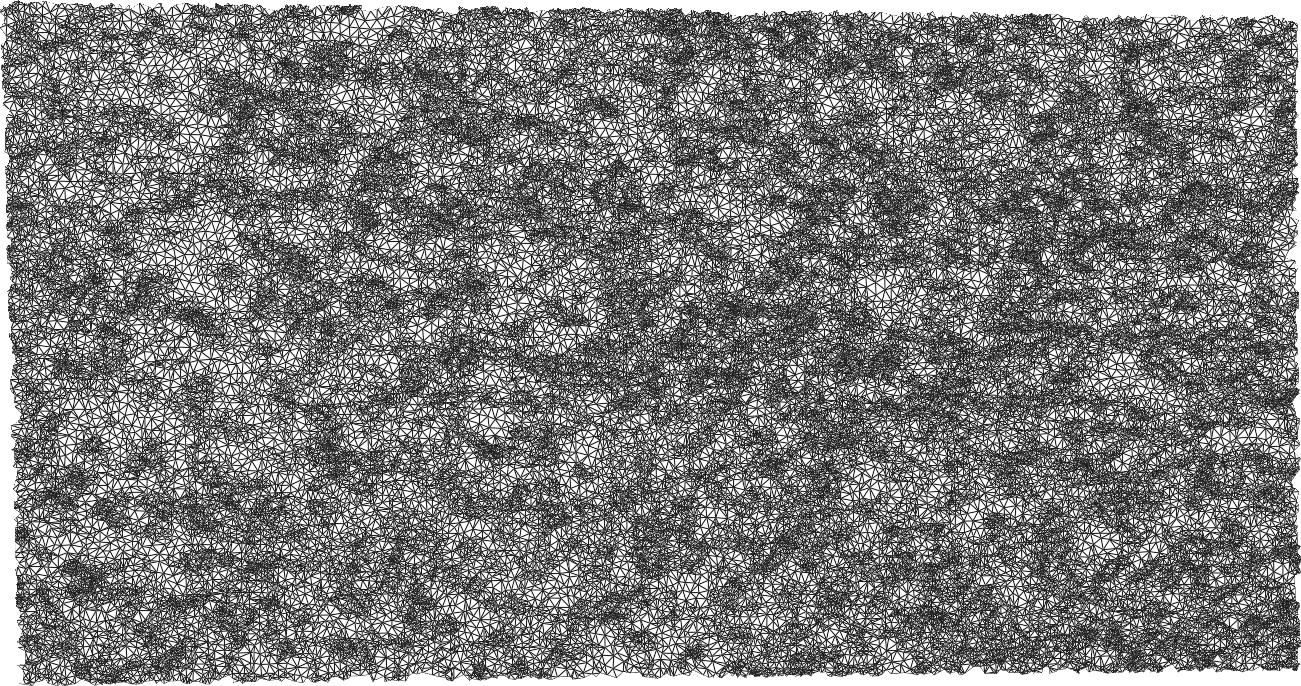
\includegraphics[width=\linewidth]
		{data/acquired_meshes/ILATO_1A_SM2066-HE5-60_070214_merged_GMO_r1_n4_v256_wireframe.png}
		\caption{wireframe}\label{ILATO:bun.a}
	\end{subfigure}
	\begin{subfigure}[b]{0.49\linewidth}
		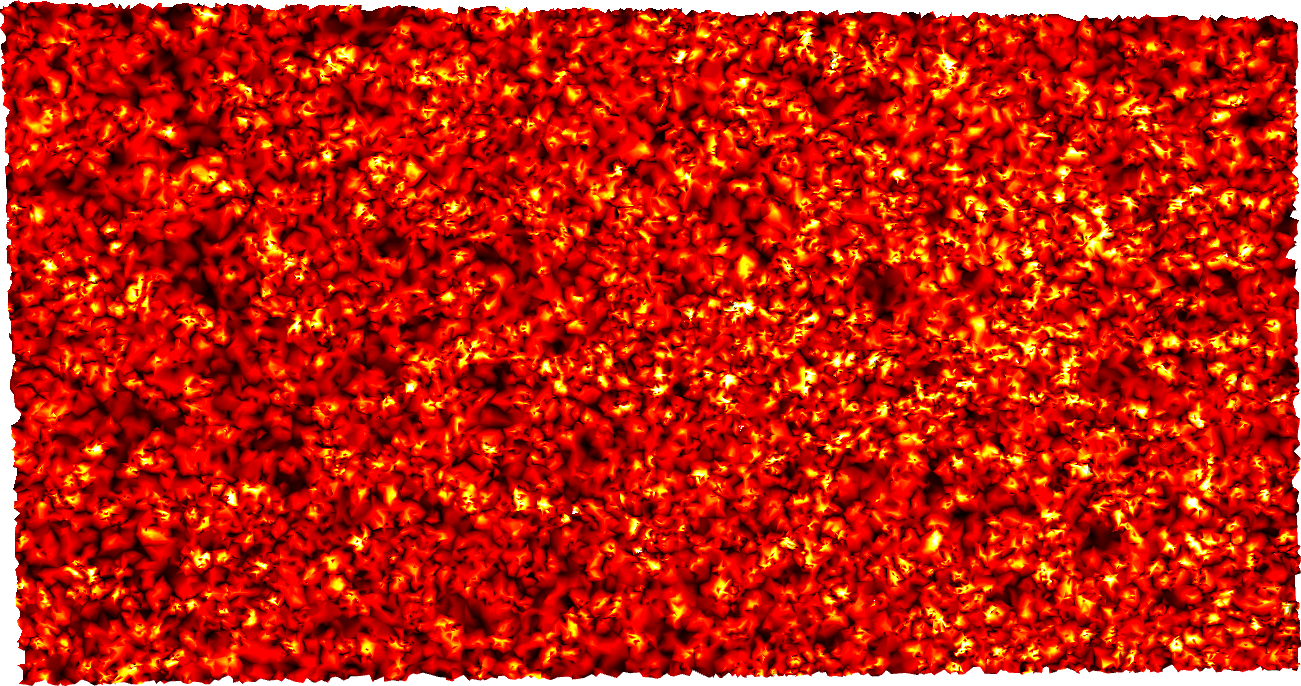
\includegraphics[width=\linewidth]
		{data/acquired_meshes/ILATO_1A_SM2066-HE5-60_070214_merged_GMO_r1_n4_v256_funcvals_0iter.png}
		\caption{$c=0$}\label{fig:buILATOn.b}
	\end{subfigure}

	\bigskip
	\begin{subfigure}[b]{0.49\linewidth}
		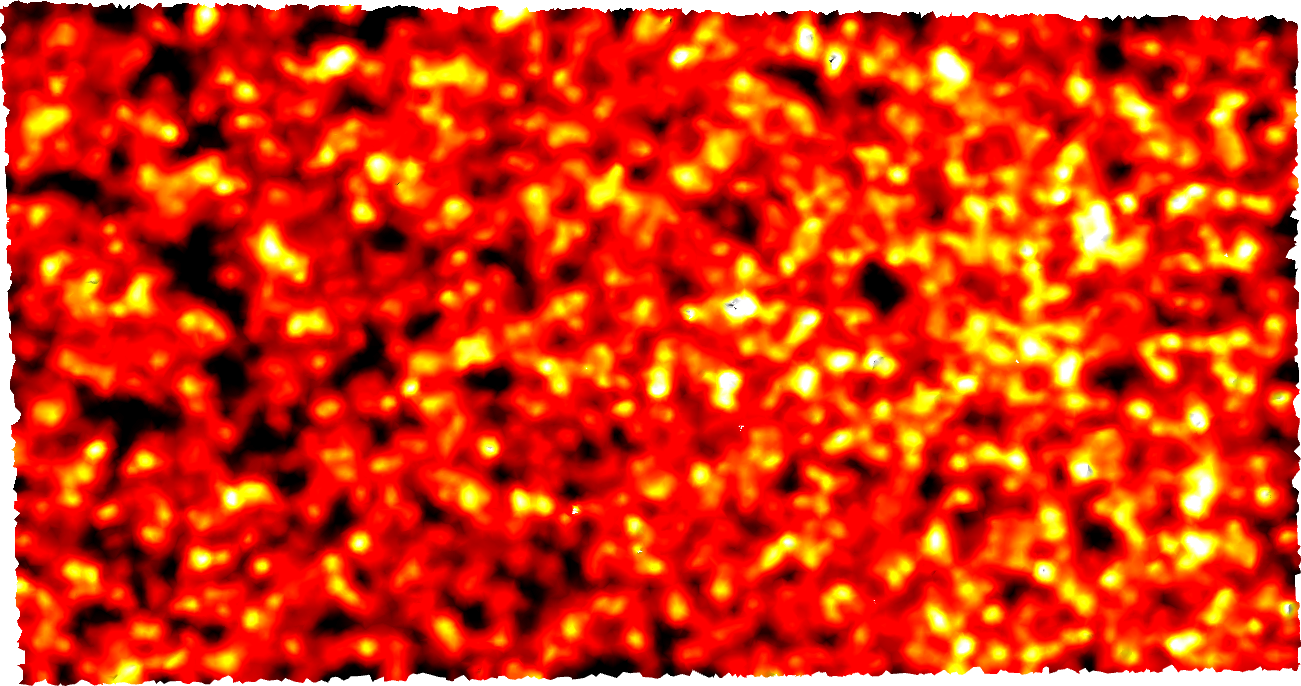
\includegraphics[width=\linewidth]
		{data/acquired_meshes/ILATO_1A_SM2066-HE5-60_070214_merged_GMO_r1_n4_v256_funcvals_1000iter.png}
		\caption{$c=1000$}\label{fig:ILATO.c}
	\end{subfigure}
	\begin{subfigure}[b]{0.49\linewidth}
		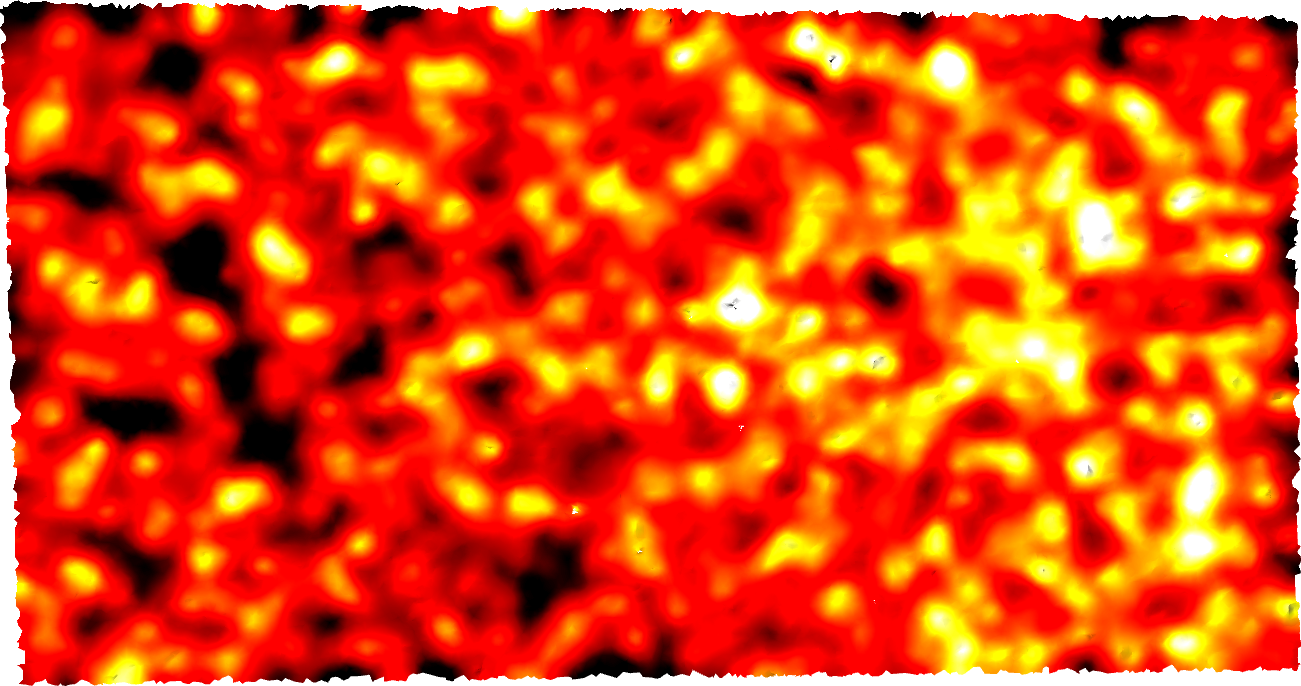
\includegraphics[width=\linewidth]
		{data/acquired_meshes/ILATO_1A_SM2066-HE5-60_070214_merged_GMO_r1_n4_v256_funcvals_3000iter.png}
		\caption{$c=3000$}\label{fig:ILATO.d}
	\end{subfigure}
\end{figure}

		\end{minipage}
	}
}

%------------------------------------------------
\frame{\frametitle{The Stanford Bunny}
	\vspace*{1cm}
	\centering
	\scalebox{1.0}{
		\begin{minipage}{\textwidth}
			\begin{figure}[ht]
	\begin{subfigure}[b]{0.32\linewidth}
		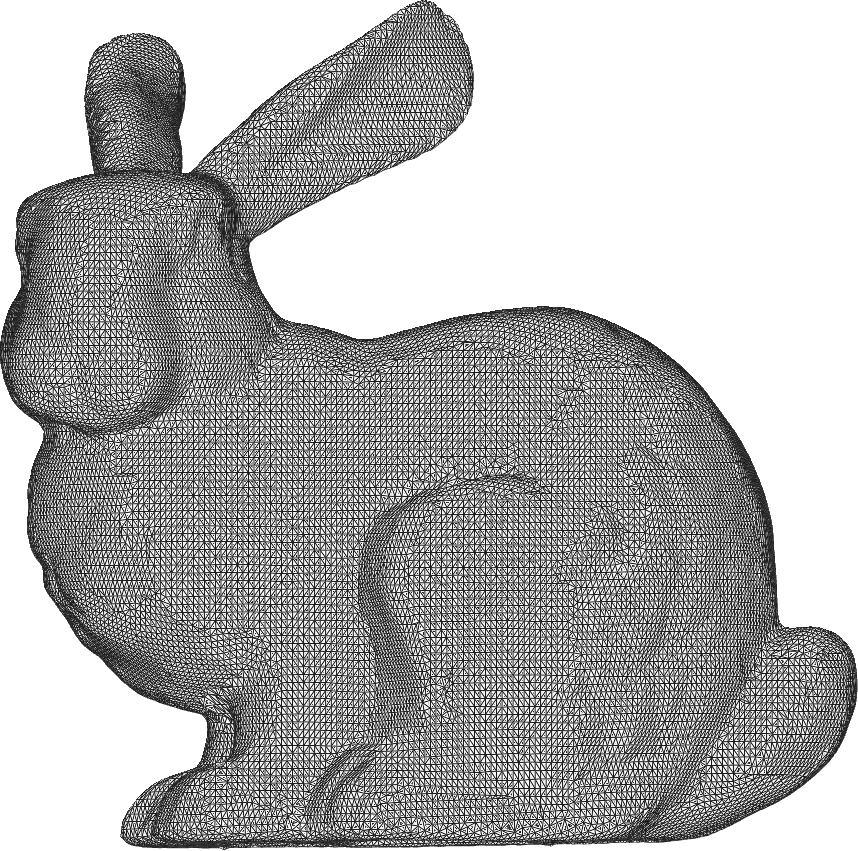
\includegraphics[width=\linewidth]
		{data/acquired_meshes/bun_zipper_edited_r1_n4_v256_wireframe.png}
		\caption{wireframe}\label{fig:bun.a}
	\end{subfigure}
	\begin{subfigure}[b]{0.32\linewidth}
		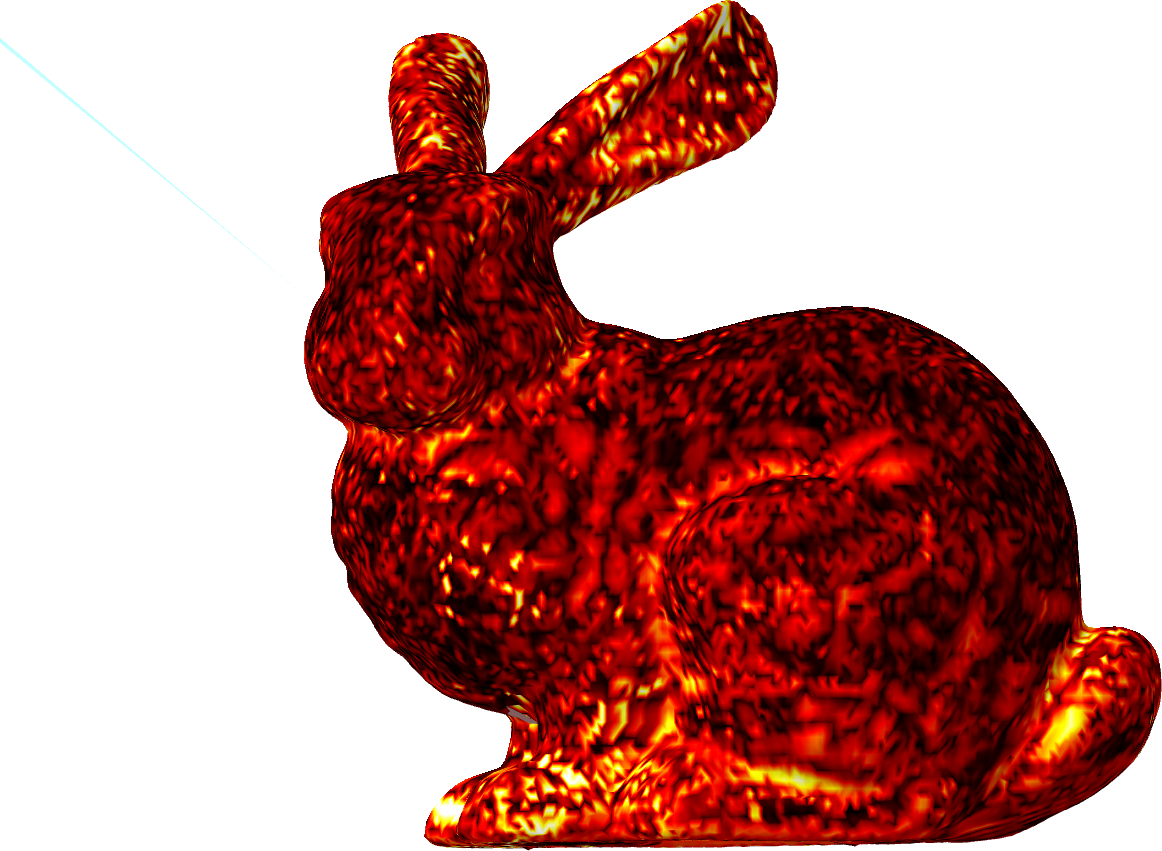
\includegraphics[width=\linewidth]
		{data/acquired_meshes/bun_zipper_edited_r1_n4_v256_funcvals_0iter.png}
		\caption{$c=0$}\label{fig:bun.b}
	\end{subfigure}
	\begin{subfigure}[b]{0.32\linewidth}
		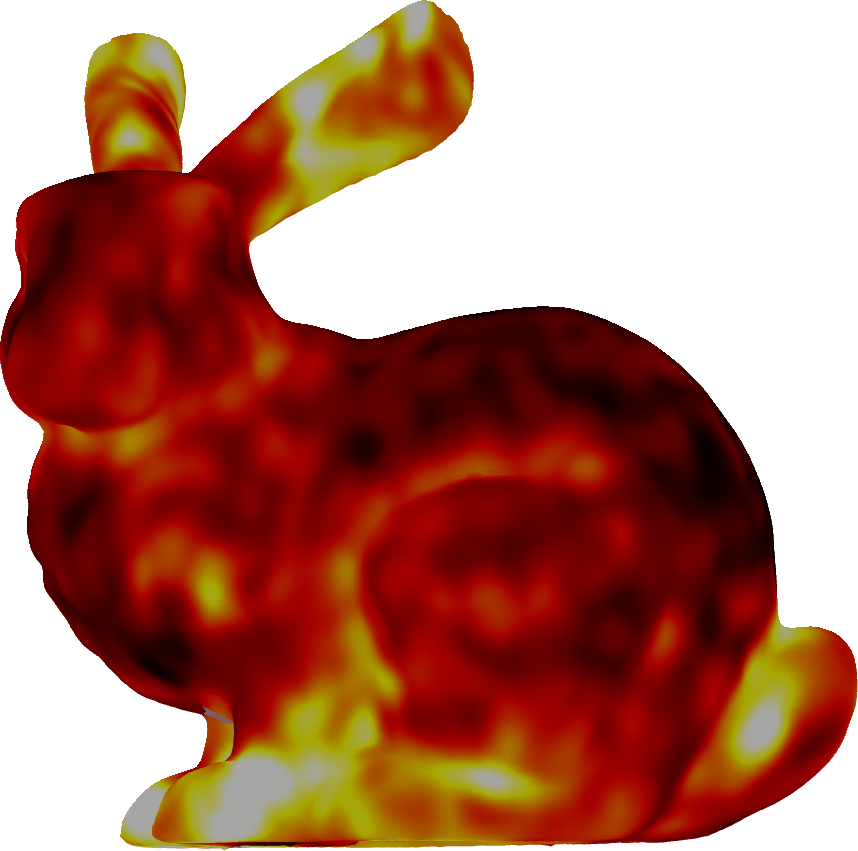
\includegraphics[width=\linewidth]
		{data/acquired_meshes/bun_zipper_edited_r1_n4_v256_funcvals_100iter.png}
		\caption{$c=100$}\label{fig:bun.c}
	\end{subfigure}
\end{figure}

		\end{minipage}
	}
}




%================================================
\subsection{Convolving with a \gls{GPGPU}}

%------------------------------------------------
\frame{\frametitle{Evaluation and Analysis of Parallel Algorithms}

Two basic timings:
\begin{align*}
	\mathit{T_s}(\hat{n}) &= \text{sequential execution time} \\%\text{The optimal sequential execution time} \\
	\mathit{T_{\rho}}(\hat{n},\,\rho) &= \text{Parallel execution time}
\end{align*}

Three essential metrics:
\begin{align*}
	\text{Speedup:}\quad&\mathit{S}(\hat{n},\,\rho) = \frac{\mathit{T_s}(\hat{n})}{\mathit{T_{\rho}}(\hat{n},\,\rho)} \\
	\text{Costs}:\quad&\mathit{C}(\hat{n},\,\rho) =\rho\cdot\mathit{T_{\rho}}(\hat{n},\,\rho) \\
	\text{Efficiency}:\quad&\mathit{E}(\hat{n},\,\rho) = \frac{\mathit{T_s}(\hat{n})}{\mathit{C}(\hat{n},\,\rho)} = \frac{\mathit{S}(\hat{n},\,\rho)}{\rho}
\end{align*}
}

%------------------------------------------------
\frame{\frametitle{Amdahl's law and the Degree of Parallelism}
	\begin{columns}[T]
		\begin{column}{.425\textwidth}
			``Degree of Parallelism'': the maximum share of operations that can be executed in parallel

			\medskip
			\begin{block}{Amdahl's law}
				Given a constant problem size $\hat{n}_{fixed}$,
				\begin{equation*}
					\lim_{\rho \to \infty} \mathit{S}(\hat{n}_{fixed},\,\rho) = 1 / q
				\end{equation*}
			\end{block}

			\medskip
			\textbf{Conclusion}: one \emph{cannot} simply add more processors in order to gain appreciable speedup!
		\end{column}
		\begin{column}{.575\textwidth}
			\includegraphics[width=1.0\textwidth]{figures/amdahlsLaw.png}
		\end{column}
	\end{columns}
}

%------------------------------------------------
%TODO: exchange experiment codes with points to notice
\frame{\frametitle{Compute Times per Experiment for increasing Convolution Counts}
	\vspace*{-4mm}
	\begin{columns}[T]
		\begin{column}{.31\textwidth}
			\centering
			\includegraphics[width=1.0\textwidth]{figures/computeTimesLinespoints.png}
		\end{column}
		\begin{column}{.69\textwidth}
			The experiment codes:
				\begin{itemize}
					\item the system
					\begin{itemize}
						\item T for the desktop
						\item M for the laptop
					\end{itemize}
					\item the algorithm variant
					\begin{itemize}
						\item P for parallel
						\item S for serial
					\end{itemize}
					\item the mesh being processed
					\begin{itemize}
						\item BS for bisected-square
						\item HT for hexagonal tessellation
						\item US for university seal
						\item FS for the flat surface
					\end{itemize}
					\item the count of points comprising the mesh.
				\end{itemize}
		\end{column}
	\end{columns}
}

%------------------------------------------------
\frame{\frametitle{Compute Times Scatter Plot}
	\vspace*{-3mm}
	\centering
	\includegraphics[width=.72\textwidth]{figures/computeTimesScatter.png}
}

%------------------------------------------------
\frame{\frametitle{Speedup}
	\vspace*{-3mm}
	\centering
	\includegraphics[width=.9\textwidth]{figures/speedup.png}
}

%------------------------------------------------
\frame{\frametitle{Efficiency}
	\vspace*{-3mm}
	\centering
	\includegraphics[width=.9\textwidth]{figures/efficiency.png}
}


%================================================
%================================================
\section[Conclusion]{Conclusion \& Outlook}

%------------------------------------------------
\frame{\frametitle{Conclusion}
	\begin{columns}
		\begin{column}{.5\textwidth}
			Filter Response:
			\begin{itemize}
				\item the filter works
				\item anisotropic behavior
				\item filter response slows down for irregular meshes
				\item errors propagate in ``unclean'' meshes
				\item efficacy diminishes with variance
			\end{itemize}
		\end{column}
		\begin{column}{.5\textwidth}
			Algorithm Performance:
			\begin{itemize}
				\item Speedups higher than 200x achieved %but not 2,500x as may have been expected
				\item Efficiency only as high as 15\% %improvements can be made
			\end{itemize}
		\end{column}
	\end{columns}
}

%------------------------------------------------
\frame{\frametitle{Outlook}
	\begin{columns}
		\begin{column}{.5\textwidth}
			New Features:
			\begin{itemize}
				\item Implement with OpenCl to include other GPGPUs
				\item Implement with OpenMP to utilize networks
				\item New user defined parameter %min edge length, discoverd by typo in original code
				\item Explicitly support feature vectors
			\end{itemize}
		\end{column}
		\begin{column}{.5\textwidth}
			Alternative Approaches:
			\begin{itemize}
				\item Using inner angles vs area for weights
				\item Explore storing edge lengths once %could not run some experiments due to memory
				\item Other smoothing methods, i.e. median
				\item Use inverse squares for interpolation
			\end{itemize}

			\bigskip
			Optimization:
			\begin{itemize}
				\item Eliminate square root function %no averaging, interpolation
				\item Improve efficiency in general %target explicit synchronization, memory pipelining
				\item Elegantly handle errors edge cases
			\end{itemize}
		\end{column}
	\end{columns}
}

%------------------------------------------------
\frame{\frametitle{Questions}
	\includegraphics[width=.8\textwidth]{questions}
	\vspace*{-3.3cm}
	\begin{center}
		\begin{LARGE}
			\textbf{Questions}
		\end{LARGE}
	\end{center}
	\vspace*{2cm}
}\fi
\end{document}
